%\documentclass[pdftex,a4paper]{scrreprt}
\documentclass[fleqn,pdftex,paper=a4,pagesize,11pt,numbers=noenddot]{scrreprt}
\usepackage[intoc]{nomencl}
\usepackage[numbers]{natbib}
\usepackage{booktabs}
\usepackage{geometry}
\usepackage{multirow}
\usepackage{multicol}
\usepackage{booktabs}
\usepackage{fancyhdr}
\usepackage{array}

\usepackage[nottoc]{tocbibind}

\usepackage[T1]{fontenc}
\setcounter{tocdepth}{3}


\usepackage{algorithmicx}
\usepackage{algorithm}
\usepackage{algpseudocode}
\floatname{algorithm}{Procedure}

%\usepackage[automark]{scrpage2}
\usepackage{cite}

\usepackage[dvips]{color}
\usepackage{epsfig}
\usepackage{grffile}
\usepackage{epstopdf}
\usepackage{ae}

\usepackage{amsmath}
\usepackage{amssymb}
\usepackage{amsfonts}
\usepackage{amsthm}
\usepackage{mathtools}

\usepackage{float}
\usepackage{graphics}
\usepackage{graphicx, subfigure}
\setcounter{lofdepth}{2}
\graphicspath{{/Volumes/workspace/studium/bachelorarbeit/thesis/media/}}
\newcommand{\rulesep}{\unskip\ \vrule\ }
\newcommand{\rpm}{\sbox0{$1$}\sbox2{$\scriptstyle\pm$}
  \raise\dimexpr(\ht0-\ht2)/2\relax\box2 }

\usepackage{titlepage}

\usepackage{appendix}

\usepackage{pstricks}

\pagestyle{headings}

\usepackage{ifthen}
\makenomenclature
\makeindex
\setlength{\nomlabelwidth}{.25\hsize}
%\renewcommand{\nomlabel}[1]{#1 \dotfill}
\setlength{\nomitemsep}{-\parsep}

\renewcommand{\nomgroup}[1]{%
\renewcommand{\makelabel}[1][]{##1}
\item[~]
\ifthenelse{\equal{#1}{A}}{\item[\lARGE\textbf{Abbreviations}]}{
\ifthenelse{\equal{#1}{B}}{\item[\lARGE\textbf{Operators and Symbols}]}{
\ifthenelse{\equal{#1}{C}}{\item[\lARGE\textbf{Superscripts and Subscripts}]}{
\ifthenelse{\equal{#1}{D}}{\item[\lARGE\textbf{Domains and boundaries}]}{
\ifthenelse{\equal{#1}{E}}{\item[\lARGE\textbf{Kinematics}]}{
\ifthenelse{\equal{#1}{F}}{\item[\lARGE\textbf{Stresses and constitutive laws}]}{
\ifthenelse{\equal{#1}{G}}{\item[\lARGE\textbf{Governing equations}]}{
\ifthenelse{\equal{#1}{H}}{\item[\lARGE\textbf{Contact Mechanics}]}{
\ifthenelse{\equal{#1}{I}}{\item[\lARGE\textbf{Numerical methods}]}{}}}}}}}}}
\item[~]
\let\makelabel\nomlabel
}


\DeclareMathOperator{\tr}{tr}
\DeclareMathOperator{\Div}{Div}
\DeclareMathOperator{\Lin}{Lin}
\DeclareMathOperator{\divnew}{div}
\DeclareMathOperator{\Grad}{Grad}
\DeclareMathOperator{\tonew}{to}
\DeclareMathOperator{\innew}{in}
\DeclareMathOperator{\on}{on}
\DeclareMathOperator{\subjectnew}{subject}


\makeindex

%%%%%%%%%%%%%%%%%%%%%%%%%%%%%%%%%%%%%%%%%%%%%%%%%%%%%%%%%%%%%%%%%%%%%%%
%%%%%%%%%%%%%%%%%%%%%%%%%%%%             %%%%%%%%%%%%%%%%%%%%%%%%%%%%%%
%%%%%%%%%%%%%%%%%%%%%%%%%%%% end of file %%%%%%%%%%%%%%%%%%%%%%%%%%%%%%
%%%%%%%%%%%%%%%%%%%%%%%%%%%%             %%%%%%%%%%%%%%%%%%%%%%%%%%%%%%
%%%%%%%%%%%%%%%%%%%%%%%%%%%%%%%%%%%%%%%%%%%%%%%%%%%%%%%%%%%%%%%%%%%%%%%

\usepackage{hyperref}
\usepackage{bookmark}
\usepackage{multirow}
\usepackage{rotating}

%%
\usepackage[framemethod=tikz]{mdframed}
\usetikzlibrary{calc}
\usepackage{kantlipsum}

%\usepackage{dingbat}%\eye and \leftpointright

\newcounter{error}[chapter]
\renewcommand*\theerror{\thechapter.\arabic{error}}
\tikzset{
errorsymbol/.style={%
    rectangle,draw=blue,
   ,scale=2,overlay}}

\tikzstyle{line} = [ draw, -latex']  
\usetikzlibrary{calc}

\tikzset{
 lampsymbol/.style={%
   ,scale=2,overlay}}

\newmdenv[hidealllines=true,backgroundcolor=blue!5,%
 frametitle={\stepcounter{error}Comman~Programming~Error~\theerror},
 frametitlefont=\color{blue!80!black}\bfseries,
 skipabove=\topsep,skipbelow=\topsep,nobreak,
 leftmargin=.3cm,rightmargin=.3cm, innerleftmargin=2cm,
 singleextra={\path let \p1=(P), \p2=(O) in ($(\x2,0)+0.5*(2,\y1)$) node[errorsymbol] {aaa};},%
]{error}


\newmdenv[nobreak,middlelinewidth=.8pt,
 frametitlefont=\bfseries,
 leftmargin=.3cm,rightmargin=.3cm, innerleftmargin=2cm,
 skipabove=\topsep,skipbelow=\topsep,
 singleextra={\path let \p1=(P), \p2=(O) in ($(\x2,0)+0.5*(2,\y1)$) node[ lampsymbol] {.h};
                          \draw[line width=.8pt,white,] ($(O|-P)+(.2cm,0)$) -- ($(P)-(.2cm,0)$); 
                          \draw[line width=.8pt,white,] ($(O)+(.2cm,0)$) -- ($(P|-O)-(.2cm,0)$);
    },%
]{bbbb}

\newcommand{\infobox}[1]{\begin{bbbb}[frametitle={Reference to NS-EOF namespaces}]#1\end{bbbb}}



%%

%%
\usepackage{lscape}
%\usepackage{adjustbox}
%%

\usepackage{etex}
\newcounter{alteSeitenzahl}

\usepackage{tikz}
\usetikzlibrary{shapes,arrows,chains}
\usepackage{xcolor}

\usepackage{graphicx}
%\usepackage[usenames,dvipsnames,svgnames,table]{xcolor}

\usepackage{dirtree}
\usepackage{epstopdf}
\usepackage{textcomp}
\usepackage[final]{listings}
\definecolor{lightgray}{rgb}{.7,.7,.7}
\definecolor{gray}{rgb}{.4,.4,.4}
\definecolor{darkblue}{rgb}{0,0,.3}

\newcommand{\noi}{\noindent}
\newcommand{\noii}{\vspace{3mm}\noindent}

\newcommand{\abl}[2]{\frac{\partial\,#1}{\partial\,#2}}
\newcommand{\abll}[2]{\frac{\partial^2\,#1}{\partial\,#2^2}}
\newcommand{\ave}[1]{\left\langle #1 \right\rangle}
\newcommand{\new}[1]{\textcolor{red}{#1}}

%\lstset{
%showstringspaces=false,
%extendedchars=true,
%frameround=fttt,
%frame=single,
%upquote=true,
%breaklines=true
%}

\newcommand{\ke}{$k$-$\varepsilon$}

\newcommand{\xmll}[2]{
    \lstset{
numberstyle=\tiny,%5
basicstyle={\ttfamily},%
    language=xml,
    %tabsize=3,
    %frame=lines,
    %caption=Test,
    %label=code:sample,
    %frame=shadowbox,
    %rulesepcolor=\color{gray},
    %xleftmargin=20pt,
    %framexleftmargin=15pt,
    frame=single,
    keywordstyle=\color{blue}\bf,
    commentstyle=\color{OliveGreen},
    stringstyle=\color{red},
    numbers=left,
    numberstyle=\tiny,
    %numbersep=5pt,
    breaklines=true,
    showstringspaces=false,
    %basicstyle=\footnotesize,
    emph={food,name,price},emphstyle={\color{magenta}}}
\lstinputlisting[firstline=#2]{#1}}

\newcommand{\bashh}[2]{
    \lstset{
numberstyle=\tiny,%5
basicstyle={\ttfamily},%
    language=xml,
    %tabsize=3,
    %frame=lines,
    %caption=Test,
    %label=code:sample,
    %frame=shadowbox,
    %rulesepcolor=\color{gray},
    %xleftmargin=20pt,
    %framexleftmargin=15pt,
    frame=single,
    keywordstyle=\color{blue}\bf,
    commentstyle=\color{OliveGreen},
    stringstyle=\color{red},
    numbers=left,
    numberstyle=\tiny,
    %numbersep=5pt,
    breaklines=true,
    showstringspaces=false,
    %basicstyle=\footnotesize,
    emph={food,name,price},emphstyle={\color{magenta}}}
\lstinputlisting[firstline=#2]{#1}}

\begin{document}





%\pagestyle{useheadings}
\pagenumbering{roman}


\thesistype{Project Report}
\author{Marten Lienen, Peter M\"unch, Walter Simson, Josef Winter}
\matno{ a}
\title{$k$-$\varepsilon$ Turbulence Model}
\tutor{ b}{ c}


\maketitle
\newpage
\thispagestyle{empty}
\quad
\newpage

\tableofcontents
\printnomenclature
\newpage

\setcounter{alteSeitenzahl}{\value{page}}
\pagenumbering{arabic}

\chapter{Introduction} % (fold)
\label{cha:introduction}

% Peter


The k-$\varepsilon$-turbulence model was implemented part of the lab course 'Turbulent Flow Simulation on HPC-Systems'. For the purpose of efficiency, stability and testing a literature study was performed and following aspects have been considered and added to the existing code framework:

\begin{itemize}
\item wall models
\item new scenarios
\item PETSc optimization
\item adaptive time stepping
\item restart point \& initialisation of the pressure field in PETSc.
\end{itemize}

\noi Results were compared to literature: the wall near velocities (linear and logarithmic layer) matched well with the expected profile. The terms of the transport equations were predicted qualitatively well due to the chosen wall model (Chien).

\noii Furthermore comparisons of the DNS results with measurement results were conducted for a backwards facing step scenario and a flow around a cylinder (Karman Vortex Street).
High emphasis was put on the stochastic evaluation. To be able to simulate a flow around a circle the possibility of importing any arbitrary geometry was implemented.

\noii Extensive thoughts were made how to structure the files of each project in an optimal way (usability \& later clarity).

% chapter introduction (end)
%!TEX root = ./../projectReport.tex

\nomenclature[A]{CPP}{Closest point projection}
\nomenclature[A]{FE}{Finite element}
\nomenclature[A]{FEM}{Finite element method}

\chapter{Turbulence modeling with \ke\, model} % (fold)
\label{cha:turbulence_modeling_with_k_epsilon_model}

This section will give a short introduction to the basic equations solved for in the underlying code: the k-$\varepsilon$ model as a method to model the Reynolds stress tensor will be focused on. To conclude, stability aspects of the model at the wall near region will be mentioned.  

\section{Governing equations} % (fold)
\label{sec:governing_equations}

In general, resolving turbulent structures in time and space in detail is not necessary and also often not possible due to limiting computational resources.
Thus, turbulent behavior of a flow has to be modelled.
Since turbulent behavior is characterized by fluctuations of the flow quantities, they are splitted up as the sum of its mean and the fluctuations around it (Reynolds averaging). This yields exemplarilly for the velocity
\begin{equation}
	u_i(\underline{x},t) = \langle u_i \rangle (\underline{x},t) + u^{\prime}_i(\underline{x},t)
\end{equation}
Therein the operator $\langle \cdot \rangle$ denotes the mean, and the operator $\cdot^{\prime}$ the fluctuation of the respective quantity. Reynolds averaging in the context of incompressible flows is necessary for all velocity components, the pressure and the density.

\section{RANS equations} % (fold)
\label{sec:rans_equations}
Applying this approach to the dimensionless Navier-Stokes-equations and the continuity equation for incompressible flows yields the Reynolds-Averaged Navier-Stokes-equation (RANS):
\begin{equation}\label{eq:conti}
	\abl{\langle u_i \rangle}{x_i} = 0
\end{equation}
and
\begin{equation}
	\label{eq:RANS}
	\abl{\langle u_i \rangle}{t} + \langle u_j \rangle \abl{\langle u_i \rangle}{x_j} = -\frac{1}{\rho} \abl{\langle p \rangle}{x_i}+\frac{1}{Re} \abll{\langle u_i \rangle}{x_j}-\abl{\langle u_i^{\prime}u_j^{\prime} \rangle}{x_j}.
\end{equation}
For the sake of simplicity, the mean operator $\ave{\cdot}$ will not be written in the following since all quantities are averaged. Compared to the Navier-Stokes-equation for laminar flows, on the right hand side of equation \eqref{eq:RANS} the divergence of the Reynolds stress tensor (RST) $\langle -u_i^{\prime}u_j^{\prime} \rangle$ occurs. This term leads to a closure problem and thus has to be modelled.

\noii This can be done by using the physical analogy between molecular and turbulent friction. Dimensional analysis yields for the RST
\begin{equation}
	\label{eq:RST}
	\langle -u_i^{\prime}u_j^{\prime} \rangle = 2\nu_T S_{ij} - \frac{2}{3} k \delta_{ij},
\end{equation}
where $\nu_T$ refers to the turbulent viscosity, $k$ to the turbulent kinetic energy (TKE) and $\delta_{ij}$ to the Kronecker delta.
Inserting equation \eqref{eq:RST} into equation \eqref{eq:RANS} finally yields
\begin{equation}
	\label{eq:RANSmodified}
	\abl{u_i}{t}+\abl{u_i\,u_j}{x_j}=-\frac{1}{\rho}\,\abl{P}{x_i}+2\,\abl{}{x_j}\left( \left(\nu+\nu_T\right)\,S_{ij} \right)+f_i,
\end{equation}
with $f_i$ denoting an additional term for volume forces compared to the RANS equation \eqref{eq:RANS}. Furthermore, it can be shown that
\begin{equation}
	\begin{split}
		\frac{P}{\rho} &= \frac{p}{\rho}+\frac{2}{3}\,k \\
		S_{ij}         &= \frac{1}{2}\left(\abl{u_i}{x_j}+\abl{u_j}{x_i}\right)
	\end{split}
\end{equation}
holds for $P$ and $S_{ij}$. 

\noii Further modelling is necessary to determine the turbulent viscosity $\nu_T$. During the project phase, the approach of $k$-$\varepsilon$ modelling was chosen for that purpose. Therefore, two additional transport equations for the turbulent kinetic energy $k$ and the dissipation $\varepsilon$ have to be solved.
% subsubsection rans_equations (end)

\section{k-$\varepsilon$ transport equations} % (fold)
\label{sec:k_epsilon_transport_equations}

Dimensional analysis yields for the TKE
\begin{equation}
	k = \frac{1}{2} \ave{u_i^{\prime}u_j^{\prime}}
\end{equation}
where $\ave{u_i^{\prime}u_j^{\prime}}$ denotes the trace of the RST. Based on the RANS equation \eqref{eq:RANS} and the continuity equation for incompressible flows, a transport equation for $k$ can be derived.
It can be written as
\begin{equation} \label{tkeTransport}
	\abl{k}{t} + u_i\,\abl{k}{x_i}
	=
	\abl{}{x_i}\left(  B_k \abl{k}{x_i} \right) 
	-
	\varepsilon
	+
	F,
\end{equation}
with
\begin{equation}
	\begin{split}
		B_k &= \nu + \frac{\nu_T}{\sigma_k},\\
		F   &= 2\,\nu_T\,S_{i,j}S_{i,j}.
	\end{split}
\end{equation}
The first term on the left side therein denotes the material derivative of the TKE. Change in TKE can occur by either diffusion (first term on the right side), dissipation (second term on the right side) or production (third term on the right side). As will be seen in the following, the dissipation term can also be generalized to a reaction term.

\noii A transport equation for the dissipation $\varepsilon$, which also occurs in the TKE transport equation \eqref{tkeTransport}, can be derived mathematically. This yields
\begin{equation}
	\begin{split}
		\abl{\varepsilon}{t} + u_i\,\abl{\varepsilon}{x_i}
		&=
		\abl{}{x_i}\left( B_\varepsilon \abl{\varepsilon}{x_i} \right) 
		-
		C_{\varepsilon 2}\,\frac{\varepsilon^2}{k}
		+
		C_{\varepsilon 1}\,F
	\end{split}
\end{equation}
with
\begin{equation}
	\begin{split}
		B_\varepsilon = \nu + \frac{\nu_T}{\sigma_\varepsilon}
	\end{split}
\end{equation}
where $F$ is similarly defined as in \eqref{tkeTransport}. The interpretation of the single terms is analogous to the ones in the TKE-equation. 

\noii The introducing the time scale $T = k/\varepsilon$ (see \citep{adams2015}) yields for the respective transport equation:

\begin{alignat}{3} \label{eq:keTransport00}
		\abl{k}{t} + u_i\,\abl{k}{x_i}
		&=
		\abl{}{x_i}\left(  B_k \abl{k}{x_i} \right) 
		-
		\frac{1}{T}\,k
		&&+
		F, \\ \label{eq:keTransport01}
		\underbrace{\abl{\varepsilon}{t} + u_i\,\abl{\varepsilon}{x_i}}_{1}
		&=
		\underbrace{\abl{}{x_i}\left( B_\varepsilon \abl{\varepsilon}{x_i} \right)}_{2} 
		-
		\underbrace{C_{\varepsilon 2}\,\frac{1}{T}\,\varepsilon}_{3}
		&&+
		\underbrace{C_{\varepsilon 1}\,F}_{4}.
\end{alignat}

\noii Terms $1$, $2$, $3$ and $4$ can be interpeted as the material derivative, dissipation term, reaction term and production term respectively, as mentioned before. For \textit{k}-$\varepsilon$ models the turbulent viscosity can be calculated from the two new variables as
\begin{align}
	\nu_T = C_\mu\,\frac{k^2}{\varepsilon}.
\end{align}


% subsubsection k_epsilon_transport_equations (end)

% subsection governing_equations (end)


\section{Modification 1: Low-Reynolds models for wall near region} % (fold)
\label{sec:modification_1_low_reynolds_models_for_wall_near_region}


When solving the transport equations for $k$ and $\varepsilon$ as presented in equations \eqref{eq:keTransport00} and \eqref{eq:keTransport01}, stability problems at the wall near region can arise. For that reason, near wall models are necessary. They damp several terms of the $\varepsilon$ transport equations. The adapted transport equations can be written as

\begin{alignat}{4} \label{eq:keTransport02}
		\abl{k}{t} + u_i\,\abl{k}{x_i}
		&=
		\abl{}{x_i}\left(  B_k \abl{k}{x_i} \right) 
		-
		\frac{1}{T}\,k
		&&+
		F
		&&&-
		D, \\ \label{eq:keTransport03}
		\underbrace{\abl{\varepsilon}{t} + u_i\,\abl{\varepsilon}{x_i}}_{1}
		&=
		\underbrace{\abl{}{x_i}\left( B_\varepsilon \abl{\varepsilon}{x_i} \right)}_{2} 
		-
		\underbrace{C_{\varepsilon 2}\,f_2\,\frac{1}{T}\,\varepsilon}_{3}
		&&+
		\underbrace{C_{\varepsilon 1}\,f_1\,F}_{4}
		&&&+
		E.
\end{alignat}
The turbulent viscosity is defined as
\begin{align}
\label{eq:nut}
	\nu_T = C_\mu f_\mu \frac{k^2}{\varepsilon}.
\end{align}
Five model constants $C_{\mu}, \sigma_k, \sigma_{\epsilon}, C_{\epsilon 1}, C_{\epsilon 2}$ and five parameters $f_{\mu}, f_1, f_2, D, E$ can be identified in equations \ref{eq:keTransport02}, \ref{eq:keTransport02} and \ref{eq:nut}. The model constants are choosen as proposed in~\citep{fan1993} as
\begin{align}\label{equ:constants}
    C_{\mu} = 0.09 \qquad
    \sigma_k = 1.0 \qquad
    \sigma_{\epsilon} = 1.3 \qquad
    C_{\epsilon 1} = 1.4 \qquad
    C_{\epsilon 2} = 1.8 .	
\end{align}

\noii For the damping parameters, different models have been implemented. In the following, a table with the implemented models and the respective terms for the parameters is shown (see also~\citep{fan1993}).

\begin{adjustbox}{width=\textwidth,totalheight=\textheight,keepaspectratio}
    \begin{tabular}{| >{$}l<{$} | >{$}c<{$} | >{$}c<{$} | >{$}c<{$} | >{$}c<{$} | >{$}c<{$} |}
      \hline
      \text{} & f_{\mu} & f_1 & f_2 & \text{D} & \text{E} \\
      \hline
      \text{Jones and Launder}
      & \exp{\left\lbrack \frac{-2.5}{\left( 1+\frac{R_t}{50} \right)} \right\rbrack}
      & 1.0
      & 1-0.3 \exp{\left(-R_t^2\right)}
      & 2 \nu \left( \abl{\sqrt{k^2}}{y} \right)
      & 2 \nu \nu_T \left( \abll{u}{y} \right)^2 \\
      \text{Chien}
      & 1-\exp{\left( -0.0115 y^+ \right)}
      & 1.0
      & 1-\left( 2/9 \right) \exp{\left\lbrack -\left( \frac{R_t}{6} \right)^2 \right\rbrack}
      & 2 \nu \frac{k}{y^2}
      & -2 \nu \frac{\epsilon}{y^2} \exp{\left( -0.5y^+ \right)} \\
      \text{Lam and Bremhorst}
      & \left\lbrack 1-\exp{\left( -0.0165 R_y \right)} \right\rbrack^2 \left( 1+ \frac{20.5}{R_t} \right)
      & 1+\left(\frac{0.05}{f_{\mu}} \right)^3
      & 1-\exp{\left( -R_t^2 \right)}
      & 0.0
      & 0.0 \\
      \text{Myong and Kasagi}
      & \left\lbrack 1+\frac{3.45}{\sqrt{R_t}} \right\rbrack \times \left\lbrack 1-\exp{\left( -\frac{y^+}{5} \right)} \right\rbrack
      & 1.0
      & \left\lbrack 1-\frac{2}{9} \exp{-\left( \frac{R_t}{6} \right)^2} \right\rbrack \times \left\lbrack 1-\exp{\left( -\frac{y^+}{5} \right)} \right\rbrack
      & 0.0
      & 0.0 \\
      \text{Nagano and Hishida}
      & \left\lbrack 1-\exp{\left( -\frac{y^+}{26.5} \right)} \right\rbrack^2
      & 1.0
      & 1-0.3\exp{\left( -R_t^2 \right)}
      & 2 \nu \left( \abl{\sqrt{k^2}}{y} \right)^2
      & 2 \nu \nu_T \left( 1-f_{\mu} \right) \left( \abll{u}{y} \right)^2 \\
      \text{Fan}
      & 0.4 \frac{f_w}{\sqrt{R_t}}+\left( 1-\frac{f_w}{\sqrt{R_t}} \right) \left\lbrack 1- \exp{\left( -\frac{R_y}{42.63} \right)} \right\rbrack^3
      & 1.0
      & \left\{ 1.0 - \frac{0.4}{1.8} \exp{\left\lbrack -\left( \frac{R_t}{6} \right)^2 \right\rbrack} \right\} f_w^2
      & 0.0
      & 0.0 \\
      \hline
    \end{tabular}
\end{adjustbox}

\noii Therein, for the model of Fan, an additional parameter $f_w$ is necessary. It is defined as
\begin{equation}
f_w = 1 - \exp{\left\{ -\frac{\sqrt{R_y}}{2.30} + \left( \frac{\sqrt{R_y}}{2.30} - \frac{R_y}{8.89} \right) \left\lbrack 1-\exp{\left( -\frac{R_y}{20} \right)} \right\rbrack^3  \right\}}.
\end{equation}
Furthermore, the turbulent Reynolds numbers necessary to determine the factor are defined as
\begin{equation}
	\begin{split}
		R_y = \frac{\sqrt{k\,h}}{\nu} \qquad R_t = \frac{k^2}{\nu\,\varepsilon},	
	\end{split}
\end{equation}
where $h$ denotes the closest wall distance. How to change the chosen wall model can be found in section~\ref{sec:configuration_file}.

\infobox{
nseof::flowmodels::ke::KEStencilF
}

% subsection modification_1_low_reynolds_models_for_wall_near_region (end)

\section{Modification 2: Limitations in transport equations} % (fold)
\label{sec:modification_2_limitation_of_source_and_reaction_terms_in_transport_equtions}


In addition to that, another option to improve stability is implemented. Proposed by \citep{kuzmin2007}, this method aims to avoid negative diffusion and reaction coefficients.


% subsection modification_2_limitation_of_source_and_reaction_terms_in_transport_equtions (end)

\section{Modified equations and discretization} % (fold)
\label{sec:modified_equations_and_discretization}

In addition to the RANS-equations (\ref{eq:conti} and \ref{eq:RANSmodified}), following two equations, which contain both modifications, are solved by NS-EOF:

\begin{alignat}{5} \label{eq:keTransport04}
		\abl{k}{t} + u_i\,\abl{k}{x_i}
		&=
		\abl{}{x_i}\left(  B_k \abl{k}{x_i} \right) 
		-
		f_3\,\frac{1}{T}\,k
		&&+
		F
		&&&-
		D, \\ \label{eq:keTransport05}
		\underbrace{\abl{\varepsilon}{t} + u_i\,\abl{\varepsilon}{x_i}}_{1}
		&=
		\underbrace{\abl{}{x_i}\left( B_\varepsilon \abl{\varepsilon}{x_i} \right)}_{2} 
		-
		\underbrace{C_{\varepsilon 2}\,f_2\,\frac{1}{T}\,\varepsilon}_{3}
		&&+
		\underbrace{C_{\varepsilon 1}\,f_1\,F}_{4}
		&&&+
		E,
\end{alignat}
\noii with
\begin{align}
	f_2&=\left\{\begin{array}{cl} f_2, & \mbox{if }f_2 / T>0 \\ 0, & \mbox{else} \end{array}\right.,
	\\
	f_3&=\left\{\begin{array}{cl} 1, & \mbox{if } 1/T>0 \\ 0, & \mbox{else} \end{array}\right..
\end{align}

\noii For information about implementational aspects of the \textit{k}-$\varepsilon$ model and how it is included in the overall algorithm to solve the flow problem see the next chapter.

% subsection modified_equations_and_discretization (end)

% chapter turbulence_modeling_with_k_epsilon_model (end)


\chapter{Numerics and algorithm} % (fold)
\label{cha:algorithm}

Please keep in mind the meaning of the 'exponents' $\left.\cdot^\circ\right.$ and $\left.\cdot^+\right.$: variable at this timestep and at the next timestep.

\section*{Discretization}

Following discretization was chosen to solve the equations given in \ref{eq:conti}, \ref{eq:RANSmodified}, \ref{eq:keTransport04} and \ref{eq:keTransport05}:
\begin{itemize}
\item spacial discretization: finite difference method
\item time discretization: mixed treatment (pressure implicit with backward Euler; velocity, turbulent kinetic energy and dissipation rate explicit - see Griebel \citep{griebel1998}).
\end{itemize}
The discretization of the two additional transport equations is straight forward, with only two additional derivatives to be discretized, which are identical for both equations (here only presented in x-direction):

\begin{align*}
\left[\abl{}{x}\left(A\,\abl{B}{x}\right)\right]_{i,j,k}
= \frac{2}{\Delta x_{i,j,k}}
\left( 
\frac{(\Delta x_{i+1,j,k}\cdot A_{i,j,k}+\Delta x_{i,j,k}\cdot A_{i+1,j,k}) \cdot (B_{i+1,j,k}-B_{i,j,k})}{(\Delta x_{i+1,j,k}+\Delta x_{i,j,k})^2} \right.\\
-\left.
\frac{(\Delta x_{i,j,k}\cdot A_{i-1,j,k}+\Delta x_{i-1,j,k}\cdot A_{i,j,k}) \cdot (B_{i,j,k}-B_{i-1,j,k})}{(\Delta x_{i,j,k}+\Delta x_{i-1,j,k})^2} 
\right)
\end{align*}

\begin{align*}
\left[\abl{(u\,B)}{x}\right]_{i,j,k}
= 
\frac{1}{\Delta x_{i,j,k}}\left(
u_{i,j,k}\frac{\Delta x_{i+1,j,k}B_{i,j,k}+\Delta x_{i,j,k}B_{i+1,j,k}}{\Delta x_{i+1,j,k}+\Delta x_{i,j,k}}\right.
\\-\left.
u_{i-1,j,k}\frac{\Delta x_{i,j,k}B_{i-1,j,k}+\Delta x_{i-1,j,k}B_{i,j,k}}{\Delta x_{i,j,k}+\Delta x_{i-1,j,k}}
\right)
\end{align*}
with:
\begin{center}
\begin{tabular}{lll}
Equ. \ref{eq:keTransport04}: & $A=B_k$           & $B=k$\\
Equ. \ref{eq:keTransport05}: & $A=B_\varepsilon$ & $B=\varepsilon$
\end{tabular}
\end{center}

\newpage
\section*{Timestep}
A first guess for the new timestep is calculated with the same equation as implemented for the algebraic turbulence model:

\begin{align}
\Delta t < \min\left\lbrace
\nu_{max}^{-1}\cdot
\left( 
\frac{1}{\Delta x^2}+
\frac{1}{\Delta y^2}+
\frac{1}{\Delta z^2}
\right)^{-1}
,
\frac{\Delta x}{|u_{max}|},
\frac{\Delta y}{|v_{max}|},
\frac{\Delta z}{|w_{max}|}
\right\rbrace
\end{align}
with:
\begin{align}
\nu_{max}=\nu_M = 2\cdot\left( \nu+\nu_T \right)
\end{align}
It was examined whether the diffusion terms of the $k$- and $\epsilon$- transport equations are more critical than the one from the momentum equation ($\nu_K$ and $\nu_E$). It has, however, proven that the diffusion rate of the momentum equation ($\nu_m$) is the highest:
\begin{align}
\nu_K = \nu+\frac{\nu_T}{\sigma_k}<\nu_M\\
\nu_E = \nu+\frac{\nu_T}{\sigma_\varepsilon}<\nu_M
\end{align}
The timestep is reduced by so much that in the next timestep there are no negative $k$ and $\varepsilon$\footnote{The user can specify whether a certain error for $k$ and $\varepsilon$ is acceptable or not in the configuration file.}.

\noii Big increases in the timestep were programmatically prevented:
\begin{align*}
\Delta\,t^+=\min{(\Delta\,t^\circ\cdot 1.1,\,\Delta\,t^+_{guess})}
\end{align*} 
for stability reasons.

\newpage
\section*{Algorithm}
Following steps are performed in our program to solve the RANS with the help of the \ke\, model in each timestep (for a simplified graphical representation of the algorithm see figure~\ref{fig:alg}):
\begin{itemize}
\item[1.] Estimate $\Delta t$
\item[2.] Calculate $k$ and $\varepsilon$ (first step):
\begin{align}\label{KK1}
K^\circ&=
\abl{}{x_i}\left(\nu_t\,\abl{k}{x_i}\right)
-
\abl{(u_i\cdot k)}{x_i}
+
\frac{1}{2}\nu_t
(\,S_{i,j} \cdot S_{i,j})
-
\varepsilon
\\\label{EE1}
E^\circ&=\frac{c_\varepsilon}{c_\mu}\cdot
\abl{}{x_i}\left(f_\mu\,\nu_T\,\abl{\varepsilon}{x_i}\right)
-
\abl{(u_i\cdot \varepsilon)}{x_i}
+
\frac{c_1\,f_1}{2}k
(\,S_{i,j} \cdot S_{i,j})
-
c_2\,f_2\frac{\varepsilon^2}{k}
\end{align}\vspace{-0.5cm}



\item[3.] Calculate temporal $k$ and $\varepsilon$ (second step):
\begin{align}
k^* &= k^\circ + \Delta t \cdot K^\circ\\
\varepsilon^* &= \varepsilon^\circ + \Delta t \cdot E^\circ
\end{align}\vspace{-0.5cm}

Check for validity and if necessary adjust timesteps.

\item[4.] Make temporal $k^*$ and $\varepsilon^*$ final ($k^+$ and $\varepsilon^+$)

\item[5.] Calculate $F_i^\circ$:
\begin{align}
F_i^\circ=u_i^\circ+\Delta t\left(-\abl{u_i^\circ\,u_j^\circ}{x_j} +2\,\abl{}{x_j} \left( \,\left(\nu+\nu_T^\circ\right)S_{ij}^\circ\right)+f_i^\circ  \right)
\end{align}
\item[6.] Solve the Pressure-Poission-Equation for $(p^+/\rho)$ $\rightarrow$ \textsc{PETSc}:
\begin{align}
\frac{1}{\Delta t} \abl{F_i^\circ}{x_i}  =
\frac{\partial^2 (p^+/\rho)}{\partial x_i\,\partial x_i}
\end{align}
\item[7.] Calculate velocities $u_i^+$:
\begin{align}
u_i^+
=F_i^\circ-\frac{\Delta t}{\rho}\,\abl{(p^+/\rho)}{x_i}
\end{align}
\item[8.] Calculate eddy viscosity $\nu_T^\circ$:
\begin{align}
\nu_{t}^+=c_\mu\frac{\left(k^+\right)^2}{\varepsilon^+}
\qquad\qquad\text{and}\qquad\qquad
l_m = \sqrt{\frac{3}{2}} c_\mu\frac{\left(k^+\right)^{3/2}}{\varepsilon^+}
\end{align}
\vspace{-0.5cm}
\item[9.] Calculate wall near correction factors ($f_1$, $f_2$, $f_2$, $f_{\mu}$, $D$ and $E$)
\item[10.] Calculate additional useful variables: velocity fluctuation $u'$ and pressure $p$:
\begin{align}
u'=\sqrt{\frac{2}{3}k}\qquad\qquad
\frac{{p}}{\rho}=\frac{{P}}{\rho}-\frac{2}{3}\,K=\frac{{P}}{\rho}-u'u'
\end{align}
\end{itemize}





\clearpage
\begin{center}

\begin{figure}[!htb]

% =================================================
% Set up a few colours
\colorlet{lcfree}{green}
\colorlet{lcnorm}{blue}
\colorlet{lccong}{red}
% -------------------------------------------------
% Set up a new layer for the debugging marks, and make sure it is on
% top
\pgfdeclarelayer{marx}
\pgfsetlayers{main,marx}
% A macro for marking coordinates (specific to the coordinate naming
% scheme used here). Swap the following 2 definitions to deactivate
% marks.
\providecommand{\cmark}[2][]{%
  \begin{pgfonlayer}{marx}
    \node [nmark] at (c#2#1) {#2};
  \end{pgfonlayer}{marx}
  } 
\providecommand{\cmark}[2][]{\relax} 
% -------------------------------------------------
% Start the picture
\begin{tikzpicture}[%
    >=triangle 60,              % Nice arrows; your taste may be different
    start chain=going below,    % General flow is top-to-bottom
    node distance=6mm and 60mm, % Global setup of box spacing
    every join/.style={norm},   % Default linetype for connecting boxes
    ]
% ------------------------------------------------- 
% A few box styles 
% <on chain> *and* <on grid> reduce the need for manual relative
% positioning of nodes
\tikzset{
  base/.style={draw, on chain, on grid, align=center, minimum height=4ex},
  proc/.style={base, rectangle, text width=8em},
  test/.style={base, diamond, aspect=2, text width=5em},
  term/.style={proc, rounded corners},
  % coord node style is used for placing corners of connecting lines
  coord/.style={coordinate, on chain, on grid, node distance=6mm and 25mm},
  % nmark node style is used for coordinate debugging marks
  nmark/.style={draw, cyan, circle, font={\sffamily\bfseries}},
  % -------------------------------------------------
  % Connector line styles for different parts of the diagram
  norm/.style={->, draw, lcnorm},
  free/.style={->, draw, lcfree},
  cong/.style={->, draw, lccong},
  it/.style={font={\small\itshape}}
}
% -------------------------------------------------
% Start by placing the nodes
\node [proc, densely dotted, it] (p0) {input};
% Use join to connect a node to the previous one 
\node [proc, join, below=1.5cm of p0] (KoEo)  {Calc $K^\circ$ and $E^\circ$};
\node [proc, join] (p1) {set $\Delta t$ and $n=5$};

\node [test, join, below=2.5cm of p1] (adap) {$k^*<0$\\$\varepsilon^*<0$\\$n\ge 0$};

\draw[thick,black] ($(adap.north west)+(-2.0,2.5)$)  rectangle ($(adap.south east)+(4.5,-0.8)$);

%\path (adap.east) to node [near start, xshift=2.0em] {$yes$} (adap.north); 
%  \draw [->,lcnorm] (adap.east) -- ($(adap.east) + (+1.0,+0.0)$) -- ($(adap.east) + (1.0,+1.5)$) -| (adap.north);
  
  
\node [proc,above right = +1.0cm and +4.0cm of adap] (adapp)  {$\Delta t /=2$, $n-=1$}; 
  
  
\path (adap.east) to node [near start, xshift=1.0em] {$yes$} (adapp.south); 
  \draw [->,lcnorm] (adap.east)  -| (adapp.south);

\path (adapp.north) to node [near start, xshift=2.0em] {$ $} (adap.north); 
  \draw [->,lcnorm] (adapp.north) -- ($(adapp.north) + (+0.0,+0.4)$)  -| (adap.north);  

\node [proc,below left = 3cm and -3.0cm of adap] (ke1)  {Calc $k^+$ and $\varepsilon^+$};

\node [proc, below left = 3cm and +3.0cm of adap] (fgh1) {Calc $F^\circ_i$};

\path [norm] (adap) |- (fgh1);
\path [norm] (adap) |- (ke1);

\node [proc, join, below=2cm of fgh1] (loop)  {Calc $p^+$};

\draw[black,thick] ($(loop.north west)+(-1.0,0.3)$)  rectangle ($(loop.south east)+(1.0,-0.8)$);

\node [proc, join, below=2cm of loop] (t1) {Calc $u^+$};

\path [norm]  ($(loop.south east) + (-0.3,+0.0)$) -| ($(loop.south east) + (-0.3,-0.5)$) |- ($(loop.south east) + (0.7,-0.5)$) |- (loop);



% No join for exits from test nodes - connections have more complex
% requirements
% We continue until all the blocks are positioned
\node [proc, below left = 2cm and -3.0cm of t1] (p2) {Calc: $\nu_t$, $f_1$, $f_2$, $f_\mu$, $D$, $E$, $t$};


%\node [proc, join] (p3) {Dispatch message};

\path [norm] (ke1) |- (p2);
\path [norm] (t1)  |- (p2);


\node [test, join] (t2) {$t<t_{end}$};

\path (t2.west) to node [near start, xshift=-3em, yshift=-9.0em] {$yes$} (KoEo.north); 
  \draw [->,lcnorm] (t2.west) -- ($(t2.west) + (-5.0,+0.0)$) -- ($(KoEo.north west) + (-5.0,+0.3)$) -| (KoEo.north);

\draw[black,thick] ($(p1.north west)+(-7.0,1.9)$)  rectangle ($(t2.south east)+(6,-0.5)$);

\node [term, join] (p10) {exit};

\node[draw=none,fill=none] at (-1,-9.3) {PETSc};
\node[draw=none,fill=none] at (+3.9,-1.8) {Adaptive timestep};


%\node [test] (t3) {Capacity?};
%\node [test] (t4) {$k \mathbin{{-}{=}} 1$};
% We position the next block explicitly as the first block in the
% second column.  The chain 'comes along with us'. The distance
% between columns has already been defined, so we don't need to
% specify it.
%\node [proc, fill=lcfree!25, right=of p1] (p4) {Reset congestion};
%\node [proc, join=by free] {Set \textsc{mq} wait flag};
%\node [proc, join=by free] (p5) {Dispatch message};
%\node [test, join=by free] (t5) {Got msg?};
%\node [test] (t6) {Capacity?};
% Some more nodes specifically positioned (we could have avoided this,
% but try it and you'll see the result is ugly).
%\node [test] (t7) [right=of t2] {$k \mathbin{{-}{=}} 1$};
%\node [proc, fill=lccong!25, right=of t3] (p8) {Set congestion};
%\node [proc, join=by cong, right=of t4] (p9) {Close queue};

% -------------------------------------------------
% Now we place the coordinate nodes for the connectors with angles, or
% with annotations. We also mark them for debugging.
%\node [coord, right=of t1] (c1)  {}; \cmark{1}   
%\node [coord, right=of t3] (c3)  {}; \cmark{3}   
%\node [coord, right=of t6] (c6)  {}; \cmark{6}   
%\node [coord, right=of t7] (c7)  {}; \cmark{7}   
%\node [coord, left=of t4]  (c4)  {}; \cmark{4}   
%\node [coord, right=of t4] (c4r) {}; \cmark[r]{4}
%\node [coord, left=of t7]  (c5)  {}; \cmark{5}   
% -------------------------------------------------
% A couple of boxes have annotations
%\node [above=0mm of p4, it] {(Queue was empty)};
%\node [above=0mm of p8, it] {(Queue was not empty)};
% -------------------------------------------------
% All the other connections come out of tests and need annotating
% First, the straight north-south connections. In each case, we first
% draw a path with a (consistently positioned) annotation node, then
% we draw the arrow itself.
%\path (t1.south) to node [near start, xshift=1em] {$y$} (p2);
%  \draw [*->,lcnorm] (t1.south) -- (p2);
%\path (t2.south) to node [near start, xshift=1em] {$y$} (t3); 
%  \draw [*->,lcnorm] (t2.south) -- (t3);
%\path (t3.south) to node [near start, xshift=1em] {$y$} (t4); 
%  \draw [*->,lcnorm] (t3.south) -- (t4);
%\path (t5.south) to node [near start, xshift=1em] {$y$} (t6); 
%  \draw [*->,lcfree] (t5.south) -- (t6);
%\path (t6.south) to node [near start, xshift=1em] {$y$} (t7); 
%  \draw [*->,lcfree] (t6.south) -- (t7); 
% ------------------------------------------------- 
% Now the straight east-west connections. To provide consistent
% positioning of the test exit annotations, we have positioned
% coordinates for the vertical part of the connectors. The annotation
% text is positioned on a path to the coordinate, and then the whole
% connector is drawn to its destination box.
%\path (t3.east) to node [near start, yshift=1em] {$n$} (c3); 
%  \draw [o->,lccong] (t3.east) -- (p8);
%\path (t4.east) to node [yshift=-1em] {$k \leq 0$} (c4r); 
%  \draw [o->,lcnorm] (t4.east) -- (p9);
% -------------------------------------------------
% Finally, the twisty connectors. Again, we place the annotation
% first, then draw the connector
%\path (t1.east) to node [near start, yshift=1em] {$n$} (c1); 
%  \draw [o->,lcfree] (t1.east) -- (c1) |- (p4);
%\path (t2.east) -| node [very near start, yshift=1em] {$n$} (c1); 
%  \draw [o->,lcfree] (t2.east) -| (c1);
%\path (t4.west) to node [yshift=-1em] {$k>0$} (c4); 
%  \draw [*->,lcnorm] (t4.west) -- (c4) |- (p3);
%\path (t5.east) -| node [very near start, yshift=1em] {$n$} (c6); 
%  \draw [o->,lcfree] (t5.east) -| (c6); 
%\path (t6.east) to node [near start, yshift=1em] {$n$} (c6); 
%  \draw [o->,lcfree] (t6.east) -| (c7); 
%\path (t7.east) to node [yshift=-1em] {$k \leq 0$} (c7); 
%  \draw [o->,lcfree] (t7.east) -- (c7)  |- (p9);
%\path (t7.west) to node [yshift=-1em] {$k>0$} (c5); 
%  \draw [*->,lcfree] (t7.west) -- (c5) |- (p5);
% -------------------------------------------------
% A last flourish which breaks all the rules
%\draw [->,purple, dotted, thick, shorten >=1mm]
%  (p9.south) -- ++(5mm,-3mm)  -- ++(27mm,0) 
%  |- node [black, near end, yshift=0.75em, it]
%    {(When message + resources available)} (p0);
% -------------------------------------------------



\end{tikzpicture}
% =================================================
\label{fig:alg}
\caption{Algorithm}
\end{figure}

\end{center}


% subsection adaptive_time_stepping (end)

% chapter algorithm (end)
\chapter{Performance, efficiency and further modifications} % (fold)
\label{cha:performance_efficiency_and_further_modifications}

During simulations with the \ke\,model, it was seen that the maximal time step size is much smaller than the one of a DNS simulation due to high eddy viscosity (especially near the inlet) and that the simulation takes a long time to reach steady state flow. This leads to very high computational times forcing us to deal with this situation (e.g. reducing the computational time with different methods).

\noii Please note that this section also mentions further modifications not related to the topic.
 
\section{New scenarios} % (fold)
\label{sec:new_scenarios}

All scenarios work for DNS, algebraic and $k$-$\epsilon$-simulations.

\infobox{
nseof::GlobalBoundaryFactory,\\ nseof::flowmodels::ke:GlobalBoundaryFactory
}

% subsection new_scenarios (end)

\subsection*{Channel section with symmetry boundary condition} % (fold)
\label{sub:channel_section_with_symmetry_boundary_condition}

The top and the back walls of the 'channel'-scenario are replaced by free slip conditions:

\begin{equation}
\abl{u}{n}=0
\qquad
v = 0
\qquad
\left(
\abl{k}{n}=0
\qquad
\abl{\varepsilon}{n}=0
\right)
\end{equation}  

\noii A free slip condition is often imposed along a line or plane of symmetry  thereby reducing in this case the size of the domain where the flow has to be computed by a half respectively by a forth in the 2D and 3D cases \citep{griebel1998}. Symmetry is a valid assumption for a channel flow if recirculations are neglected\footnote{Recirculation cannot be captured by RANS. One would need more advanced/expensive turbulence models.}.

\noii By the way: if the x- and y-ratio of a backward facing step are specified, it is possible to simulate a 2D free jet similar flow\footnote{Free jet is not a symmetrical phenomenon. A symmetric boundary condition leads obviously to non-physical deviation in the results.}.

% subsubsection channel_section_with_symmetry_boundary_condition (end)

\subsection*{Boundary layer over flat plate} % (fold)
\label{sub:boundary_layer_over_flat_plate}

For a 2D-simulation, the top wall of the 'channel'-scenario was replaced with an opening (Neumann boundary condition).

\noii With this scenario, a boundary layer over a flat plat can be modelled provided that the height $y$ is selected big enough compared to the local boundary layer width.

\subsection*{Free} % (fold)
\label{sub:free}

In this scenario, all wall boundary conditions of the 'channel'-scenario were removed and replaced by openings.

\subsection*{Arbitrary geometric obstacles} % (fold)
\label{sub:arbitrary_geometric_obstacles}

In any scenario, an obstacle of any form (see section~\ref{sec:geometry_file}) can be placed into the middle of the flow field. In this way, the free shear flow plane wake can be modelled. The most notable example is the flow around a circle with certain repeating flow patterns behind the obstacle also known as the K\'{a}rm\'{a}n vortex street (see section~\ref{sec:karman_vortex_street_flow_around_a_cylinder_in_a_channel}).

\noii The wall distance manager (a k-D-tree implementation) was extended to handle the new scenarios and arbitrary geometries.


\noii Limitation: 2D and 1 processor.

\infobox{
nseof::geometry::GeometryManager, \\
nseof::WallDistanceManager
}

% subsubsection arbitrary_geometric_obstacles (end)

\newpage
\section{PETSc-optimization} % (fold)
\label{sec:petsc_optimization}

Marten und Walter

% subsection petsc_optimization (end)

\newpage
\section{Restart points} % (fold)
\label{sec:restart_points}

Respart points were created for the pupose of:
\begin{itemize}
\item faster convergence: starting the simulation with a good initial condition
\item security: in the case of a crash or unexpected end of a simulation.
\end{itemize}

\noii At every restart point a backup file (.bak) is created, which can be loaded at the beginning of a simulation and which is used as the initial condition by PETSc. Following variables are written to the file for each simulation type:

\newcommand{\che}{$\checkmark$}

\begin{center}

\newcolumntype{R}[1]{>{\centering\let\newline\\\arraybackslash\hspace{0pt}}m{#1}}

\begin{tabular}{l  R{2cm}R{2cm}R{2cm}}\hline
 & DNS & Algebraic & $k$-$\varepsilon$\\\hline
Pressure $p$                                    & \che & \che &  \che \\
Velocity $u_i$                                  & \che & \che & \che \\\hline
Eddy viscosity $\nu_t$                          &      & \che &  \\
Pressure + TKE $P$                              &      & \che &  \che \\\hline
Turbulent kinetic energy $k$                    &      &      & \che \\
Dissipation rate $\varepsilon$                  &      &      & \che \\
Additional $k$-source term $D$                  &      &      & \che \\
Additional $\varepsilon$-source term Factor $E$ &      &      & \che \\
Factor $f_1$                                    &      &      & \che \\
Factor $f_2$                                    &      &      & \che \\
Factor $f_3$                                    &      &      & \che \\\hline
\end{tabular}

\end{center}
It is possible also to use the backup file of a simulation type for an other one: e.g. DNS simulation can be started for a \ke\, backup file and vice versa. For the other simulation type, unknown variables are set to be zero.

\noii Please note that no interpolation function has been implemented: simulations can be only started from backup files with the same number of processors and the same mesh configuration.

\infobox{
nseof::MPIIterator.h, nseof::MPIIteratorReader.h,\\
nseof::MPIIteratorWriter.h, nseof::PetscSolver.h
}


% subsection restart_points (end)

% chapter performance_efficiency_and_further_modifications (end)
\chapter{Validation of the \ke\, model} % (fold)
\label{cha:validation_of_k_epsilon_model}

In the following section, the results of simulations with the Chien-wall-model are shown. These results were compared with the results of the algebraic turbulence model, which were created for worksheet 2, and with literature. Also the choice of the wall model was investigated.

\section{Channel flow} % (fold)
\label{sec:channel_flow}

Different cases of channel flow were performed under following conditions:

\begin{center}
\begin{tabular}{lccc}
\hline 
Re        & 1000 & 5600 & 13750\\\hline         
Uniform velocity profile $u$         & \multicolumn{3}{c}{1.0}\\
Geometry  & \multicolumn{3}{c}{100\,$\times$\,1} \\
Mesh type & \multicolumn{3}{c}{uniform} \\
Mesh      & 64\,$\times$\,128 & 64\,$\times$\,256 & 64\,$\times$\,512 \\\hline 
\end{tabular}
\end{center}

\subsubsection*{Velocities}

Figure~\ref{fig:channel-u-profile} shows the u-velocity component along the cross section for a laminar simulation, an algebraic simulation and a $k$-$\epsilon$-simulation (both for Re$=5600$). The position of measurement and time were adjusted according to the case, so that the flow profile was stationary and fully developed.

\begin{figure}[!htb]
\centering
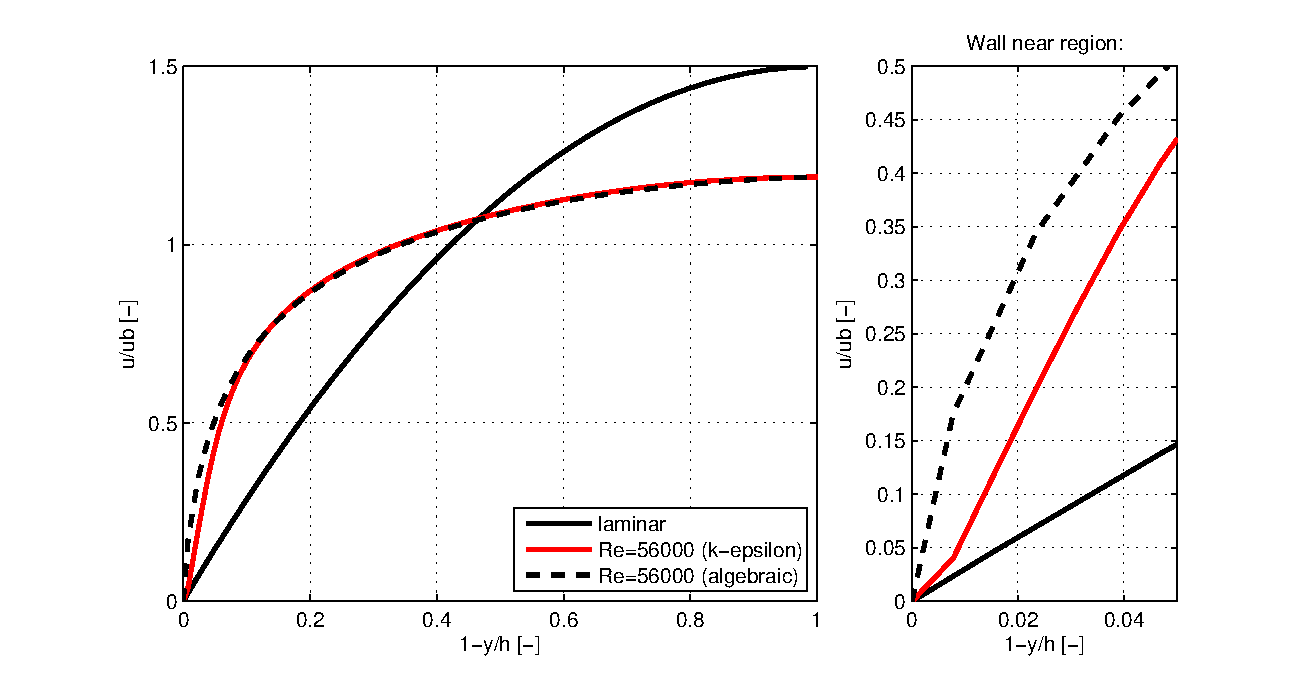
\includegraphics[width=1.0\textwidth]{FIGURES/vprofile.eps}
\caption{u-velocity profile}
\label{fig:channel-u-profile}
\end{figure} 


\noii The velocities behave as expected. In the laminar case, the velocity profile has a parabolic form with a maximum of 1.5m/s. The turbulent simulations result in lower maximum velocities (u $\le$ 1.5m/s) and in a higher slope of the velocities near the wall: the results for both turbulent models are comparable (for a more detailed comparison see the following sections).

\subsubsection*{Shear stress}

Figure~\ref{fig:channel-tau} shows the shear stress profile along the cross section for each turbulent case. The shear stress components are normalized with $\tau_{net}=\tau_v+\tau_r$:

\begin{itemize}
\item viscous stress $\tau_v=\rho\nu\abl{\ave u}{y}$
\item Reynolds stress $\tau_r=-\rho\ave{u' v'}=\rho\nu_t\abl{\ave u}{y}$
\end{itemize}

\begin{figure}[!htb]
\centering
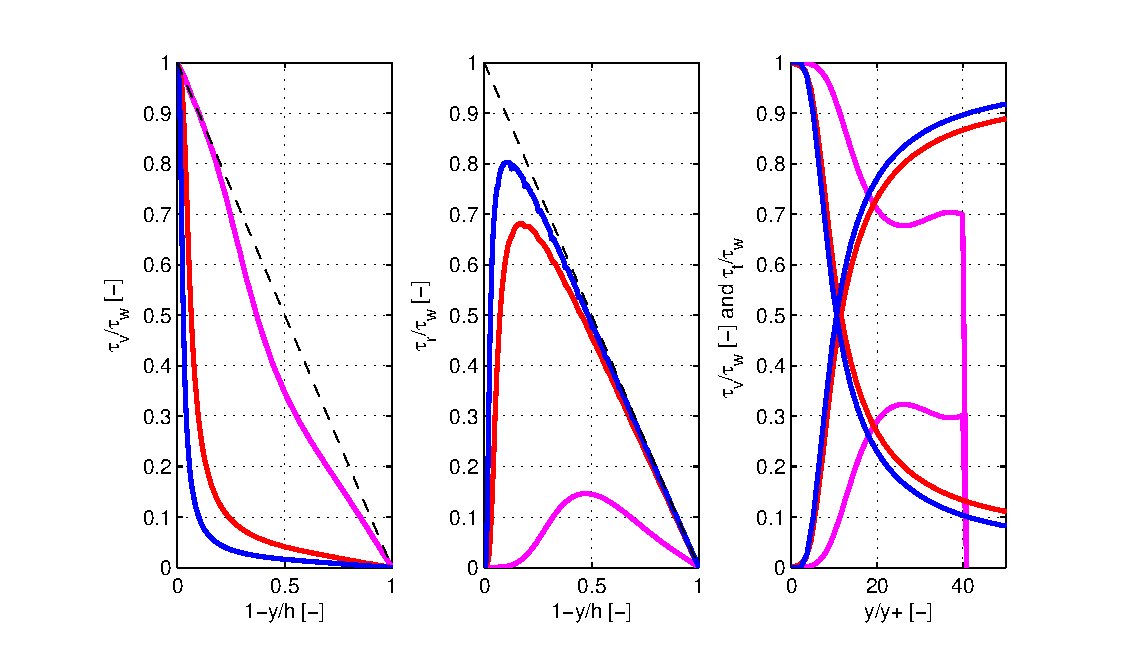
\includegraphics[width=1.0\textwidth]{FIGURES/tau.eps}
\caption{Shear stresses (viscous stress and Reynolds stress - for legend see next figure)}
\label{fig:channel-tau}
\end{figure} 

\noindent Additionally, the shear stress components are plotted over $y^+$. Self-similarity is clearly recognisable.



\subsubsection*{Comparison with the literature: velocity profile for Re=5600}\label{ssub:litkim}
Following additional values have been estimated for the turbulent Re=5600 case:
\begin{align}
u_\tau=\sqrt{\tau_w/\rho}
\qquad\qquad
l^+=\nu/u_\tau
\qquad\qquad
Re_\tau=u_\tau\cdot\delta/\nu
\end{align}
Dimensionless dimensions were created with these values and were compared with the measurement values from the literature \citep{kim1987}.

\begin{center}
\begin{tabular}{lccc}
\hline
 & Literature & Algebraic & $k$-$\varepsilon$ \\\hline
$Re_\tau$ & 180 & 352 & 170 \\
$Re_c$ & 3300 & 3329 &  3329 \\
$Re_m$ & 5600 & 5600 & 5600 \\
$u_m/u_\tau$ & 15.63 & 7.95 & 16.48 \\
$u_c/u_\tau$ & 18.20 & 9.45 & 19.59 \\
$u_c/u_m$ & 1.16 & 1.189 & 1.189 \\
$C_f = \tau_w / (0.5 \rho u_m^2)$ & 8.18$\times$10$^{-3}$ & 31.6$\times$10$^{-3}$ & 7.37$\times$10$^{-3}$ \\\hline
\end{tabular}
\end{center}

\noindent The simulated maximal velocity $u_c/u_m$ matches well with the value from the literature for both turbulent simulations. The $k$-$\epsilon$ model estimates all the $\tau_w$-related variables ($Re_\tau$, $C_f$, $u_\tau$...) much more precisely. In our last report \citep{lienen2015} we discussed, that $\tau_w$  is overestimated by the more simple model, which implies that the wall near slope of x-component of the velocity is too high.

\subsubsection*{Sublayers}\label{ssub:sublayers}

Figure~\ref{fig:sublayers_y+}-left shows the normalized velocity $w^+$  over $y^+$ and the expected velocity profile. They do match very well for high Reynolds-numbers: the linear sublayer is described exactly, the logarithmic layer shows slight discrepancy from the expectations.

\begin{figure}[!htb]
\centering
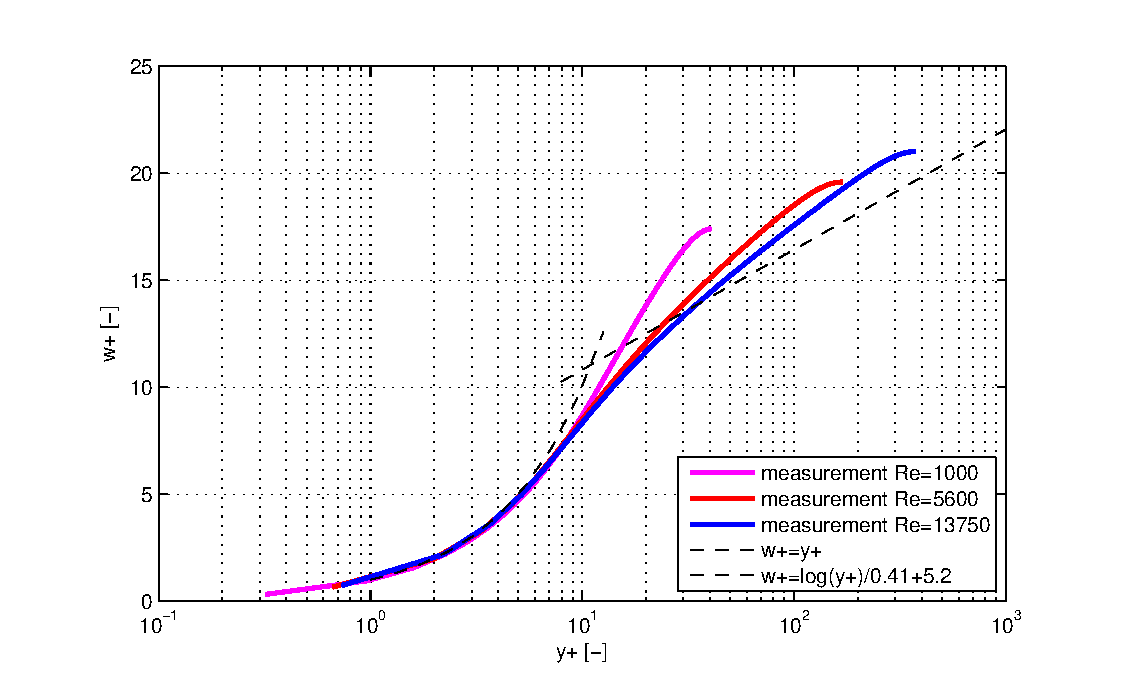
\includegraphics[trim=35 0 30 0,clip,width=0.49\textwidth]{FIGURES/wplusyplus.eps}
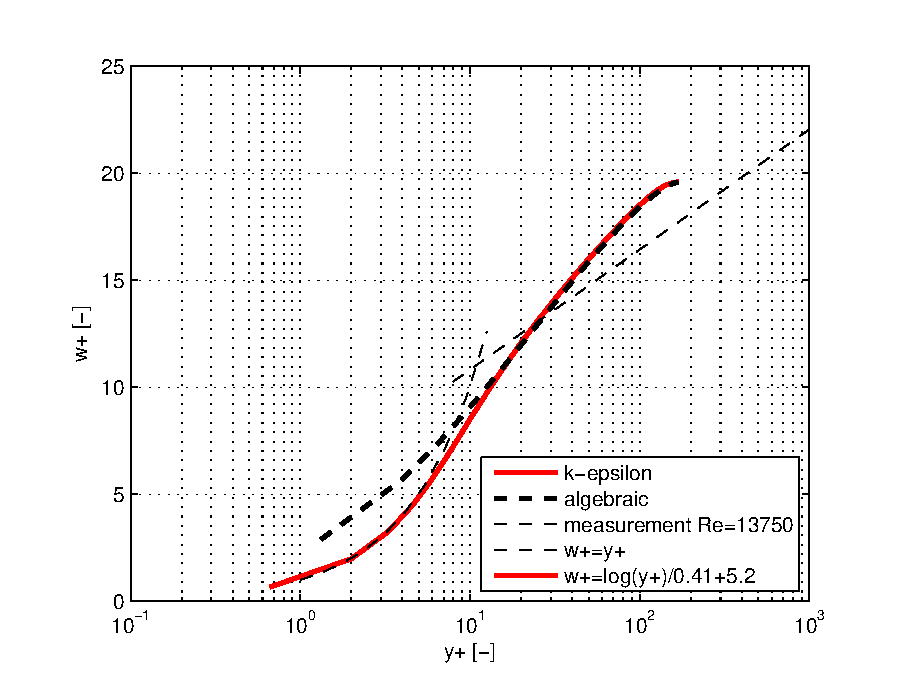
\includegraphics[trim=35 0 30 0,clip,width=0.49\textwidth]{FIGURES/avske.eps}
\caption{Sublayers: $w^+$ over $y^+$ (left: \ke\, with Re=1000, =5600 and =13750; right: Re=5600 with \ke\, and algebraic turbulence model)}
\label{fig:sublayers_y+}
\end{figure} 

\noindent Figure~\ref{fig:sublayers_y+}-right also shows a modified normalized velocity $w^+$ over $y^+$ for the algebraic turbulence model for Re=5600. In this case, $l^+$ and $u_{\tau}$ were calculated with the $\tau_w$-value estimated with the help of the \ke\, simulation: the results correspond well in the logarithmic sublayer, not that well in the linear sublayer. As expected, the slope of the velocity is too high near the wall for the algebraic model.


\subsubsection*{Comparison with the literature: TKE profile for Re=13750}

In the following the single terms in the $k$-transport equation are examined in more detail. The implemented form of this equation has the following form:

\begin{align}
\abl{k}{t} + u_i\,\abl{k}{x_i}
&=
\abl{}{x_i}\left(  B_k \abl{k}{x_i} \right) 
-
f_3\,\frac{1}{T} \, k
+
F
-
D
\end{align}
For a stationary fully developed channel flow, the equation reduces to the following form:
\begin{align}
0
&=
\underbrace{
\abl{}{y}\left(  B_k \abl{k}{y} \right) 
}_{1}
\underbrace{
-
f_3\,\frac{1}{T} \, k
-
D
}_{2}
\underbrace{+
F}_3
\end{align}
with the diffusion term (1), the dissipation term (2) and the production term (3) being in equilibrium. Figure~\ref{fig:pop_tke} shows the profile of each term in the wall near region ($y^+<50$).
\begin{figure}[!htb]
\centering
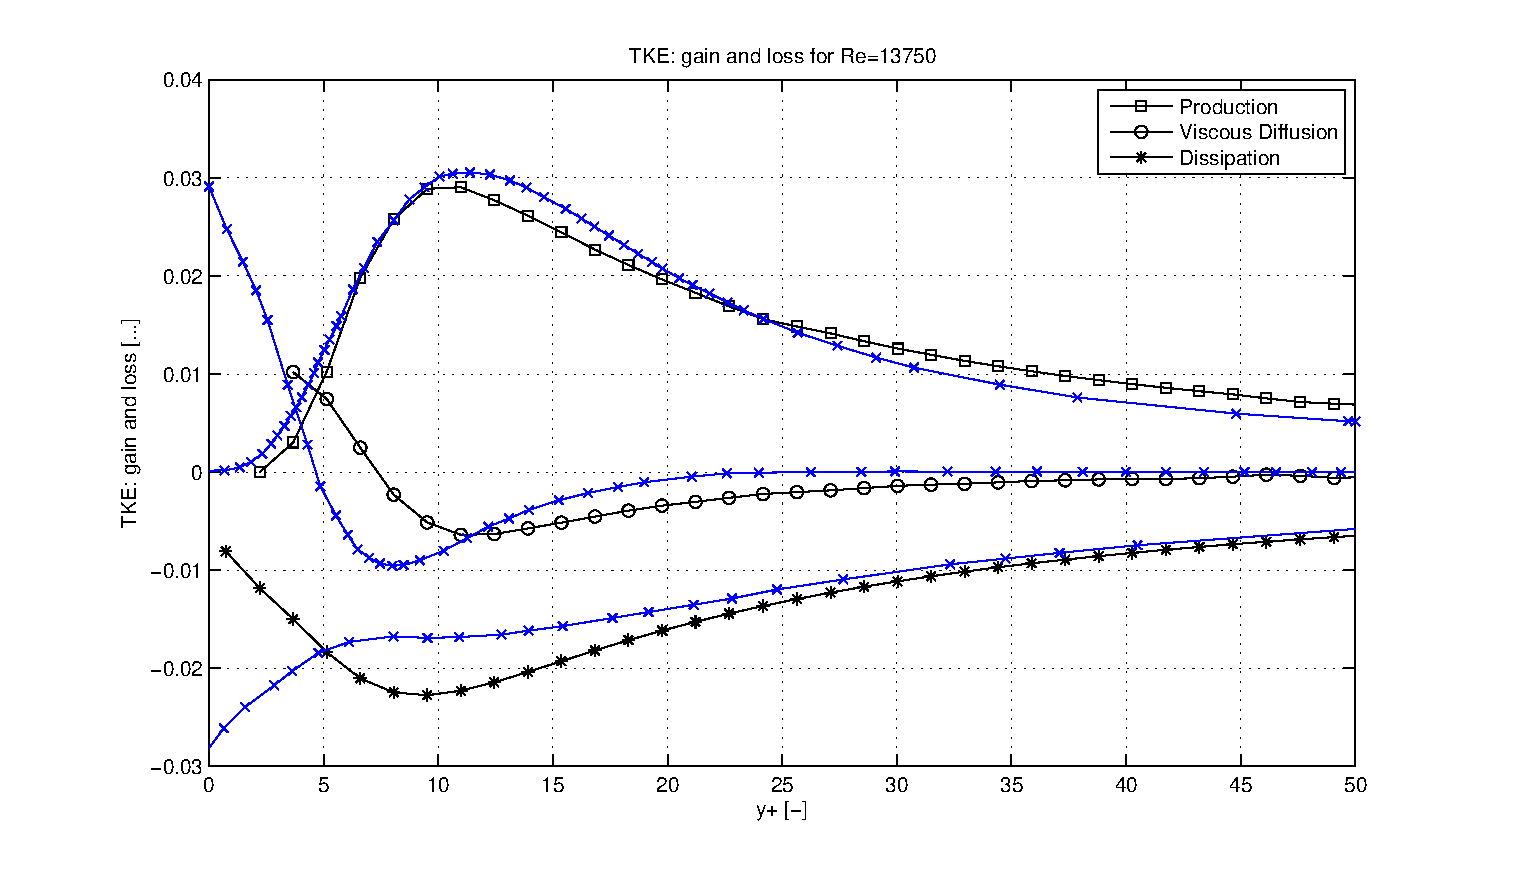
\includegraphics[trim=60 20 60 15,clip,width=0.95\textwidth]{FIGURES/tkegainloss.eps}
\caption{Terms of the TKE-transport equation for Re=13750 (in comparison with the literature \citep{pope2000} p. 285 scaled by 0.13)}
\label{fig:pop_tke}
\end{figure} 

\noii The production increases from zero at the wall and reaches its peak value well within the buffer layer, at $y^+=10$ (Pope: $y^+=12$). Around this peak, production exceeds dissipation by a factor of 1.4 (Pope: 1.8) and the excess energy produced is transported away by viscous diffusion to the wall. The dissipation is balanced by viscous transport. The peak dissipation should occur at the wall, but it does not. In the simulation, the locations of the maximal production and of the dissipation coincide.


\subsubsection*{Influence wall model}

In the case that no wall model is used during the \ke\,simulation, the profile of each term of the $k$-transport equation looks completely different. The maximum production and dissipation are at the wall. The excess energy production is transported away from the wall.

\begin{figure}[!htb]
\centering
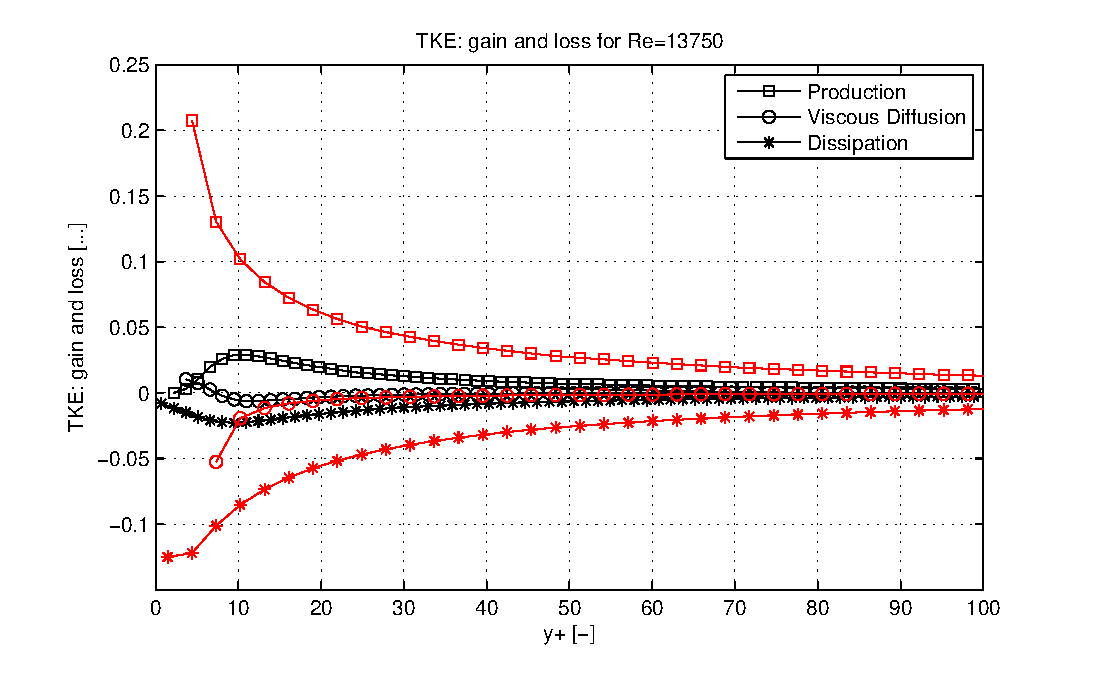
\includegraphics[width=0.95\textwidth]{FIGURES/nowallmodel.eps}
\caption{Terms of the TKE-transport equation for Re=13750 (red: without wall model; black: Chien)}
\label{fig:reswithoutwallmodel}
\end{figure} 

% subsection channel_flow (end)

\newpage
\section{Boundary layer} % (fold)
\label{sec:boundary_layer}



To further validate the implemented flow models, boundary layer simulations were performed for the laminar case and the \textit{k}-$\varepsilon$ turbulence model. The influence of wall models on the \textit{k}-$\varepsilon$ model was considered as well. The final results were compared to theoretical values.

\noii To start with, theoretical solutions for the boundary layer, over a flat plate without pressure gradient are presented. For a laminar flow and the before mentioned assumptions, an analytical solution for the boundary layer equations according to Blasius exists. It states for the boundary layer thickness
\begin{equation}
	\delta_{laminar} \approx 3.5\,\sqrt{\frac{2\nu x}{U_\infty}} = 3.5\,\sqrt{\frac{2x}{Re\,U_\infty}}.
\end{equation}
For a turbulent flow and the same assumptions the boundary layer thickness is given by
\begin{equation}
	\delta_{turbulent} \approx 0.16\,x / Re_x^{1/7},
\end{equation}
according to \citep{stemmer2015}.
Therein, the Reynolds number $Re_x$ can be calculated by
\begin{equation}
	Re_x = \frac{U_\infty x}{\nu} = U_\infty\,Re\,x.
\end{equation}
A second theoretical formula to determine the turbulent boundary layer thickness can be found in worksheet 2 of this HPC lab and states
\begin{equation}
	\delta_{turbulent} \approx 0.382\,x/Re_x^{1/5}.
\end{equation}
The simulation was performed for a plate of length $25$ and height $1$. A uniform inlet velocity profile with $U_\infty = 1.0$ was chosen. The domain was discretized by $128\times256$ cells in x- respectively y-direction. The simulation was performed for $Re=13750$. 
Furthermore, the final simulation time was chosen so that a quasi steady flow had developed. The results are shown in figure~\ref{fig:boundarylayerthickness}.

\begin{figure}[!htb]
\centering
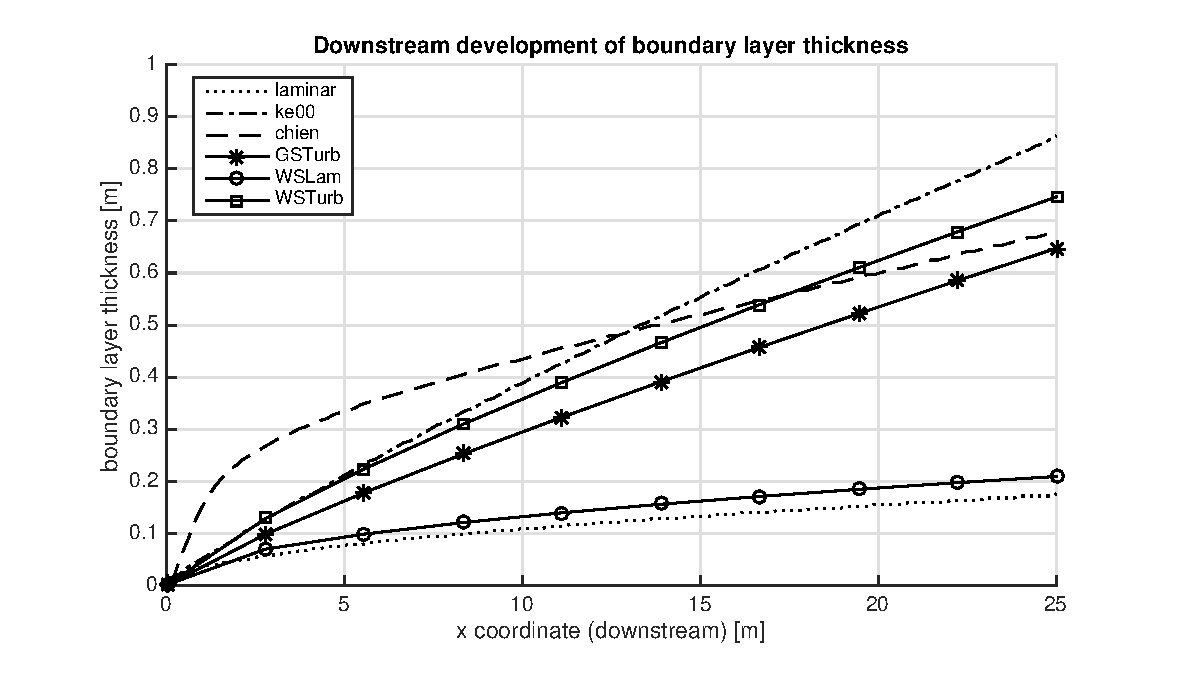
\includegraphics[width=0.78\textwidth]{FIGURES/blThickness.eps}
\caption{Boundary layer thickness over x}
\label{fig:boundarylayerthickness}
\end{figure} 


\begin{figure}[!htb]
\centering
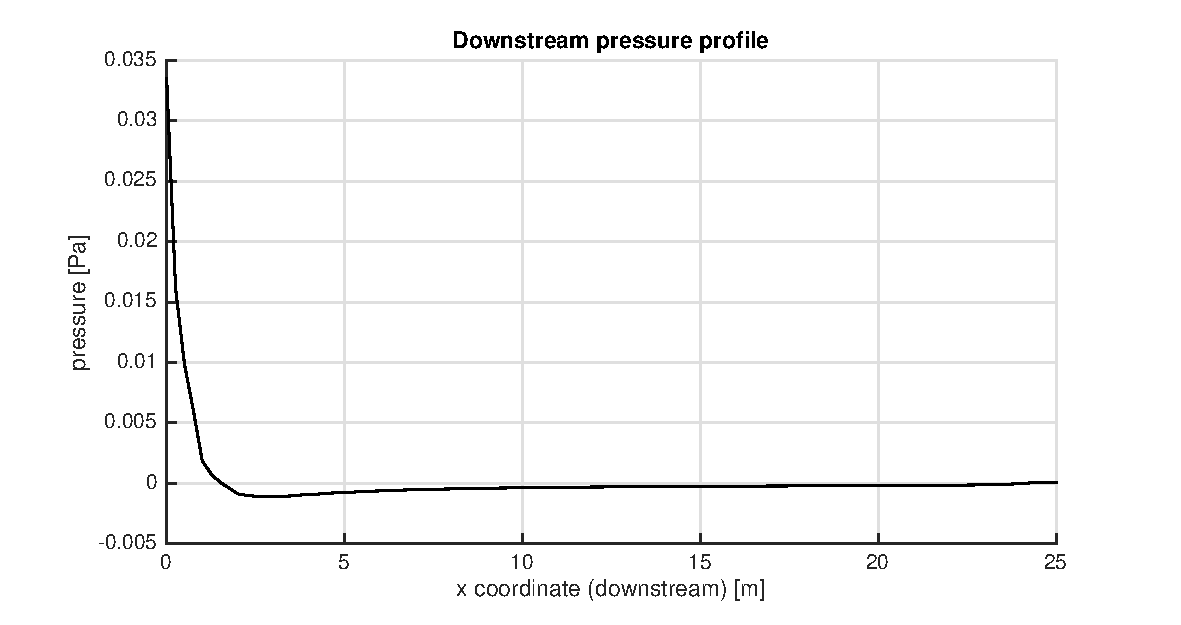
\includegraphics[width=0.78\textwidth]{FIGURES/pressure.eps}
\caption{Pressure profile at the height of $y=0.1m$}
\label{fig:boundarylayerpressure}
\end{figure} 

\noii In addition, figure~\ref{fig:boundarylayerpressure} shows exemplarily the pressure field at the last timestep for the laminar simulation. The pressure fields for both turbulent simulations are similar and are thus not shown here. Some distance behind the inlet, the pressure is nearly constant as can be seen easily. Due to that, the constant pressure assumptions made for the theoretical equations nearly match the simulation.

\noii Comparing the overall spatial developing of the boundary layer thickness of the laminar and the turbulent simulations, their boundary layer thickness profile behaves as expected. The laminar boundary layer is thinner than in turbulent cases. In addition, some distance behind the inlet the \textit{k}-$\varepsilon$ simulation without a wall model results in a thicker boundary layer. This is due to the fact, that for this model the turbulent viscosity $\nu_T$ is not damped near the wall, and thus the wall normal momentum transport is also not damped compared to Chiens model. Near the inlet this behaviour can not be detected. Presumably this is due to the influence of the inlet boundary conditions.

\noii The laminar simulation yields pretty good results when comparing to the Blasius solution. They match except for a scaling factor. For the turbulent simulations, the results deviate from the theoretical values of about $20\%$. Furthermore, the results without wall function tend to match the profile better.

\noii As expected, no transition between laminar and turbulent boundary layer could be encountered.

% subsection boundary_layer (end)

% chapter validation_of_k_epsilon_model (end)
\chapter{PETSc-Optimization} % (fold)
\label{cha:petsc}

The PETSc solver is the core of our simulation. It is responsible for actually
solving the equation system, which makes it the most time-consuming part of
running a simulation. However, it has a lot of options which could speed it up.

%%%%%%%%%%%%%%%%%%%%%

When optimizing our PETSc solver we tried multiple combinations of
preconditioned and solver for the global and local grids. Some combinations
showed a lot of promise with execution times up to 5 times faster than the
original solver. We selected the top 3 of these options with the most promise
and ran a scaling test, which quickly showed that the optimizations were not
always consistently better. Nevertheless, we performed strong scaling tests over
laminar and algebraically turbulent simulations on grids of cell size 256x64 and
512x128. The resulting plots can be found below. Left, the total poison solve
time has been plotted for all 3 variants tested along with the default
configuration, while right the speedup relative to the default configurations
has been plotted. One can extract that the execution time of the poison solver
is highly dependent the number of process, and therefore the domain
decomposition of the problem.

In general no pattern could be found to be constant, but often one of the
preconditioned variant of the fgmres-asm-preonly-ilu f proved to be faster than
the default configuration.

While scaling with algebraic turbulence models, the default configuration was
shown to be more consistent, but nevertheless, optimized solvers showed
performance in some cases. In the laminar case, although the default
configuration proved itself as stable, it was constantly beat by one of the
tested solver pre-conditioner combinations as can be seen below.  This
especially was true for jobs with 32 ranks or more.

Note: Some runs took longer than the allotted 30-minute execution time, and
therefore have no data plot for those runs. The data has never the less been
interpolated across the entire domain.

Side note: Another puzzling discovery was that the order of the conditioners and
pre- conditioners in the the petsc comandline arg script seemed to have a large
influence on PETSc's performance, at times in a drastically negative way. A
simple rearrangement of the petsc comandlind arg file quickly remedied this
issue, but as of this point, no logical reason for this is known to us.

\section{Approach}

Actually PETSc has so many options that you cannot conceivably test them
all. You can select solvers and preconditioners for the problem and when you are
working in parallel, you can also choose a different pair of solver and
preconditioner for the subdomains. If you want to go really deep, you can even
make this choice on a subdomain by subdomain basis, so that you could, for
example, use a different solver near the boundary than in the middle of a
channel scenario. On top of this there there are specific options for certain
solvers and preconditioners for fine-tuning. In view of this fact, we chose to
try an automatic approach.

\section{Preselection}

We initially hoped that a lot of the options would take continuous values. We
had the idea that we could interpret the run time of a simulation as a function
$f(p) : \mathbb{R}^{n} \rightarrow \mathbb{R}$ and use a numerical optimization
algorithm to find a configuration for minimal run time. Though the options
turned out to be mostly of the discrete variety which foiled our plan and made
this an integer optimization problem.

To combat the combinatoric explosion of option combinations, we decided to split
the optimization into two phases. In a first step we only try combinations of
solvers and preconditioners without changing specific options from their default
values because we suspect that that these have the most impact on run time over
all.

Tables \ref{fig:petsc-opt-combinations-1x1} until
\ref{fig:petsc-opt-combinations-16x4} show the resulting Poisson solving time
for all combinations of solver, preconditioner, subdomain solver and subdomain
preconditioner in a channel scenario of dimensions $5 \times 1$ with an
increasingly fine grid. The tables are of different length, because we filtered
out combinations that either diverged or did not finish in time.

Based on this ranking we chose the combination of a BiConjugate Gradient Squared
(\texttt{bcgs}) solver with an Additive Schwarz (\texttt{asm}) preconditioner on
the whole domain level and an NOP (\texttt{preonly}) solver with an incomplete
LU (\texttt{ilu}) preconditioner for further investigation because that
combination gave consistently very good results, time-wise as well as
simulation-wise. Some of the other fast combinations produced simulation
results.

\begin{table}[h]
  \tiny
  \centering
  \begin{tabular}{cccccc}
    \hline Rank & Solver & Preconditioner & Sub-Solver & Sub-Preconditioner & PETSc-Time\\ \hline

    1 & bcgs & ilu & - & - & 2.50662 \\
    2 & bcgs & jacobi & - & - & 3.85583 \\
    3 & gcr & ilu & - & - & 15.7704 \\
    4 & bcgs & bjacobi & - & - & 17.835 \\
    5 & fgmres & asm & - & - & 40.7862 \\
    6 & fgmres & gasm & - & - & 41.7788 \\
    7 & fgmres & jacobi & - & - & 47.3308 \\
    8 & gcr & asm & - & - & 49.5737 \\
    9 & gcr & gasm & - & - & 50.6497 \\
    10 & bcgs & gasm & - & - & 57.9513 \\
    11 & dgmres & asm & - & - & 75.0263 \\
    12 & gmres & gasm & - & - & 75.0506 \\
    13 & dgmres & gasm & - & - & 75.1658 \\
    14 & bcgs & bddc & - & - & 136.995 \\
    15 & cg & bddc & - & - & 137.031 \\
    16 & fgmres & bddc & - & - & 137.057 \\
    17 & dgmres & bddc & - & - & 137.127 \\
    18 & tcqmr & bddc & - & - & 137.148 \\
    19 & cr & bddc & - & - & 137.156 \\
    20 & chebyshev & bddc & - & - & 137.67 \\
    21 & bicg & bddc & - & - & 137.983 \\
    22 & lsqr & bddc & - & - & 138.319 \\
    \hline
  \end{tabular}
  \caption{PETSc-times of a $1 \times 1$ decomposition on a $128 \times 32$ grid in a $5 \times 1$ channel scenario}
  \label{fig:petsc-opt-combinations-1x1}
\end{table}

\begin{table}[h]
  \tiny
  \centering
  \begin{tabular}{cccccc}
    \hline Rank & Solver & Preconditioner & Sub-Solver & Sub-Preconditioner & PETSc-Time\\ \hline

    1 & bcgs & bjacobi & preonly & ilu & 9.91897 \\
    2 & bcgs & bjacobi & preonly & bjacobi & 10.2778 \\
    3 & bcgs & bjacobi & preonly & asm & 11.0625 \\
    4 & bcgs & asm & preonly & bjacobi & 12.0636 \\
    5 & bcgs & asm & preonly & ilu & 12.0825 \\
    6 & bcgs & jacobi & bcgs & asm & 16.8702 \\
    7 & bcgs & jacobi & bcgs & bjacobi & 16.8819 \\
    8 & bcgs & asm & preonly & jacobi & 21.4934 \\
    9 & fgmres & asm & preonly & ilu & 25.0637 \\
    10 & fgmres & bjacobi & preonly & asm & 26.5028 \\
    11 & gcr & bjacobi & preonly & ilu & 48.7232 \\
    12 & gcr & bjacobi & preonly & asm & 52.4674 \\
    13 & gcr & bjacobi & preonly & gasm & 54.3274 \\
    14 & fgmres & asm & preonly & asm & 69.0118 \\
    15 & gcr & asm & preonly & ilu & 77.1786 \\
    16 & gcr & asm & preonly & asm & 80.9108 \\
    17 & fgmres & jacobi & fgmres & asm & 86.4742 \\
    18 & fgmres & jacobi & fgmres & ilu & 86.9231 \\
    19 & fgmres & jacobi & fgmres & gasm & 88.5556 \\
    20 & fgmres & bjacobi & preonly & jacobi & 92.1365 \\
    21 & gcr & jacobi & preonly & asm & 114.156 \\
    22 & fgmres & asm & fgmres & asm & 174.54 \\
    23 & fgmres & asm & fgmres & gasm & 175.754 \\
    24 & gmres & asm & gmres & gasm & 261.226 \\
    25 & fgmres & jacobi & preonly & asm & 273.189 \\
    26 & fgmres & jacobi & fgmres & jacobi & 273.44 \\
    27 & fgmres & jacobi & preonly & gasm & 273.533 \\
    28 & gcr & jacobi & gcr & gasm & 322.474 \\
    29 & gcr & jacobi & gcr & ilu & 322.506 \\
    \hline
  \end{tabular}
  \caption{PETSc-times of a $4 \times 1$ decomposition on a $256 \times 64$ grid in a $5 \times 1$ channel scenario}
  \label{fig:petsc-opt-combinations-4x1}
\end{table}

\begin{table}[h]
  \tiny
  \centering
  \begin{tabular}{cccccc}
    \hline Rank & Solver & Preconditioner & Sub-Solver & Sub-Preconditioner & PETSc-Time\\ \hline

    1 & bcgs & asm & preonly & ilu & 4.84988 \\
    2 & bcgs & asm & preonly & asm & 5.50919 \\
    3 & bcgs & asm & preonly & bjacobi & 5.58179 \\
    4 & bcgs & bjacobi & preonly & gasm & 7.36192 \\
    5 & bcgs & jacobi & preonly & jacobi & 11.5107 \\
    6 & bcgs & jacobi & bcgs & bjacobi & 11.5891 \\
    7 & bcgs & asm & preonly & gasm & 15.0381 \\
    8 & bcgs & jacobi & preonly & bjacobi & 17.6565 \\
    9 & tfqmr & asm & preonly & ilu & 19.7188 \\
    10 & fgmres & bjacobi & preonly & ilu & 22.1083 \\
    11 & gcr & bjacobi & preonly & ilu & 22.3645 \\
    12 & gcr & asm & preonly & ilu & 23.9356 \\
    13 & gcr & asm & preonly & gasm & 24.2038 \\
    14 & gcr & bjacobi & preonly & asm & 24.2789 \\
    15 & bcgs & bjacobi & preonly & ilu & 28.4305 \\
    16 & fgmres & bjacobi & preonly & asm & 29.8764 \\
    17 & bcgs & bjacobi & preonly & bjacobi & 30.8208 \\
    18 & gcr & asm & preonly & asm & 30.8698 \\
    19 & bcgs & bjacobi & preonly & asm & 32.7116 \\
    20 & fgmres & asm & preonly & ilu & 38.1359 \\
    21 & fgmres & asm & preonly & asm & 42.3049 \\
    22 & dgmres & bjacobi & preonly & asm & 43.7851 \\
    23 & bcgs & jacobi & preonly & gasm & 58.8008 \\
    24 & bcgs & jacobi & bcgs & gasm & 59.4479 \\
    25 & fgmres & asm & fgmres & ilu & 62.1746 \\
    26 & fgmres & asm & fgmres & gasm & 70.8113 \\
    27 & dgmres & bjacobi & dgmres & bjacobi & 72.6469 \\
    28 & dgmres & asm & preonly & asm & 74.8014 \\
    29 & bcgs & asm & preonly & jacobi & 84.0214 \\
    30 & fgmres & jacobi & preonly & gasm & 103.675 \\
    31 & fgmres & jacobi & fgmres & ilu & 104.091 \\
    32 & gcr & asm & gcr & asm & 104.336 \\
    33 & fgmres & jacobi & fgmres & gasm & 104.554 \\
    34 & dgmres & bjacobi & preonly & gasm & 105.63 \\
    35 & gcr & asm & preonly & jacobi & 107.927 \\
    36 & gcr & bjacobi & preonly & gasm & 109.618 \\
    37 & bcgs & asm & bcgs & bjacobi & 110.848 \\
    38 & gcr & asm & gcr & gasm & 113.596 \\
    39 & gcr & jacobi & preonly & jacobi & 118.425 \\
    40 & fgmres & jacobi & fgmres & jacobi & 118.499 \\
    41 & gcr & jacobi & preonly & gasm & 118.593 \\
    42 & gcr & jacobi & gcr & jacobi & 118.609 \\
    43 & gcr & jacobi & gcr & ilu & 118.88 \\
    44 & gcr & jacobi & gcr & asm & 120.336 \\
    45 & fgmres & bjacobi & fgmres & ilu & 133.844 \\
    46 & gcr & jacobi & gcr & gasm & 152.573 \\
    47 & dgmres & bjacobi & dgmres & asm & 159.891 \\
    48 & fgmres & jacobi & preonly & jacobi & 167.764 \\
    49 & dgmres & asm & dgmres & bjacobi & 167.945 \\
    50 & fgmres & bjacobi & fgmres & asm & 172.146 \\
    51 & fgmres & bjacobi & fgmres & gasm & 173.781 \\
    52 & gcr & bjacobi & preonly & jacobi & 174.945 \\
    53 & gcr & bjacobi & gcr & gasm & 199.316 \\
    54 & bcgs & asm & bcgs & asm & 203.829 \\
    55 & fgmres & jacobi & preonly & ilu & 208.517 \\
    56 & fgmres & jacobi & preonly & asm & 210.162 \\
    57 & fgmres & asm & preonly & jacobi & 215.341 \\
    58 & fgmres & asm & fgmres & asm & 226.268 \\
    59 & bcgs & bjacobi & bcgs & asm & 227.503 \\
    60 & gcr & bjacobi & gcr & ilu & 230.96 \\
    61 & fgmres & bjacobi & preonly & jacobi & 242.735 \\
    62 & gcr & asm & gcr & ilu & 255.745 \\
    63 & fgmres & asm & fgmres & jacobi & 255.925 \\
    64 & gcr & jacobi & preonly & asm & 265.367 \\
    65 & gcr & jacobi & preonly & ilu & 266.239 \\
    \hline
  \end{tabular}
  \caption{PETSc-times of a $8 \times 2$ decomposition on a $256 \times 64$ grid in a $5 \times 1$ channel scenario}
  \label{fig:petsc-opt-combinations-8x2}
\end{table}

\begin{table}[h]
  \tiny
  \centering
  \begin{tabular}{cccccc}
    \hline Rank & Solver & Preconditioner & Sub-Solver & Sub-Preconditioner & PETSc-Time\\ \hline

    1 & bcgs & asm & preonly & ilu & 8.62323 \\
    2 & bcgs & asm & preonly & gasm & 9.68961 \\
    3 & fgmres & bjacobi & preonly & asm & 31.9078 \\
    4 & gcr & bjacobi & preonly & gasm & 40.1055 \\
    5 & bcgs & bjacobi & preonly & gasm & 41.4188 \\
    6 & fgmres & bjacobi & preonly & gasm & 48.6188 \\
    7 & fgmres & asm & preonly & asm & 50.7413 \\
    8 & bcgs & jacobi & preonly & bjacobi & 53.4876 \\
    9 & gcr & bjacobi & preonly & asm & 57.6915 \\
    10 & bcgs & asm & preonly & jacobi & 74.8086 \\
    11 & dgmres & asm & dgmres & gasm & 89.9251 \\
    12 & fgmres & asm & preonly & gasm & 102.872 \\
    13 & gcr & asm & preonly & asm & 114.781 \\
    14 & dgmres & asm & dgmres & asm & 119.718 \\
    15 & bcgs & jacobi & preonly & gasm & 140.977 \\
    16 & bcgs & bjacobi & preonly & ilu & 159.775 \\
    17 & bcgs & asm & preonly & bjacobi & 169.815 \\
    18 & fgmres & jacobi & fgmres & gasm & 194.687 \\
    19 & fgmres & jacobi & fgmres & jacobi & 196.768 \\
    20 & fgmres & asm & fgmres & asm & 217.465 \\
    21 & fgmres & jacobi & preonly & gasm & 245.402 \\
    22 & fgmres & jacobi & preonly & asm & 268.427 \\
    23 & gcr & asm & gcr & ilu & 272.434 \\
    24 & gcr & asm & gcr & gasm & 278.307 \\
    25 & fgmres & jacobi & preonly & jacobi & 280.382 \\
    26 & gcr & jacobi & gcr & ilu & 384.266 \\
    27 & gcr & asm & preonly & gasm & 391.81 \\
    28 & gcr & jacobi & gcr & gasm & 395.968 \\
    29 & gcr & bjacobi & gcr & gasm & 504.138 \\
    30 & gcr & bjacobi & gcr & asm & 615.469 \\
    31 & fgmres & asm & fgmres & jacobi & 767.893 \\
    32 & fgmres & bjacobi & fgmres & gasm & 817.836 \\
    \hline
  \end{tabular}
  \caption{PETSc-times of a $16 \times 2$ decomposition on a $512 \times 128$ grid in a $5 \times 1$ channel scenario}
  \label{fig:petsc-opt-combinations-16x2}
\end{table}

\begin{table}[h]
  \tiny
  \centering
  \begin{tabular}{cccccc}
    \hline Rank & Solver & Preconditioner & Sub-Solver & Sub-Preconditioner & PETSc-Time\\ \hline

    1 & bcgs & bjacobi & preonly & ilu & 5.50499 \\
    2 & bcgs & asm & preonly & ilu & 6.10181 \\
    3 & bcgs & bjacobi & preonly & bjacobi & 12.1679 \\
    4 & bcgs & jacobi & bcgs & gasm & 28.3655 \\
    5 & bcgs & asm & preonly & bjacobi & 32.8395 \\
    6 & fgmres & bjacobi & preonly & gasm & 41.2223 \\
    7 & gcr & bjacobi & preonly & ilu & 44.5088 \\
    8 & gcr & asm & preonly & asm & 48.7862 \\
    9 & fgmres & asm & preonly & gasm & 53.4382 \\
    10 & gcr & bjacobi & preonly & asm & 56.2883 \\
    11 & fgmres & asm & preonly & asm & 61.2216 \\
    12 & fgmres & bjacobi & preonly & asm & 64.4604 \\
    13 & bcgs & bjacobi & preonly & jacobi & 69.7025 \\
    14 & bcgs & jacobi & bcgs & ilu & 73.5131 \\
    15 & gcr & asm & gcr & asm & 73.723 \\
    16 & bcgs & jacobi & preonly & gasm & 73.7239 \\
    17 & bcgs & jacobi & bcgs & jacobi & 75.3447 \\
    18 & dgmres & asm & dgmres & asm & 88.7668 \\
    19 & gcr & asm & preonly & gasm & 100.861 \\
    20 & bcgs & bjacobi & preonly & gasm & 121.382 \\
    21 & fgmres & asm & fgmres & asm & 126.428 \\
    22 & gcr & bjacobi & preonly & gasm & 145.03 \\
    23 & gcr & asm & gcr & ilu & 177.899 \\
    24 & gcr & jacobi & preonly & asm & 193.614 \\
    25 & fgmres & jacobi & preonly & jacobi & 200.031 \\
    26 & gcr & jacobi & gcr & gasm & 236.216 \\
    27 & dgmres & jacobi & preonly & gasm & 240.373 \\
    28 & gcr & asm & gcr & gasm & 256.96 \\
    29 & fgmres & jacobi & fgmres & gasm & 257.051 \\
    30 & bcgs & asm & bcgs & bjacobi & 274.685 \\
    31 & bcgs & asm & bcgs & gasm & 274.848 \\
    32 & fgmres & jacobi & fgmres & jacobi & 302.701 \\
    33 & fgmres & jacobi & fgmres & asm & 316.879 \\
    34 & gcr & jacobi & preonly & ilu & 323.094 \\
    35 & gcr & asm & preonly & ilu & 324.72 \\
    36 & fgmres & asm & preonly & jacobi & 345.824 \\
    37 & gcr & bjacobi & gcr & ilu & 361.151 \\
    38 & fgmres & asm & fgmres & gasm & 378.469 \\
    39 & bcgs & jacobi & preonly & ilu & 408.646 \\
    40 & fgmres & bjacobi & fgmres & gasm & 421.003 \\
    41 & fgmres & asm & fgmres & jacobi & 442.903 \\
    42 & gcr & bjacobi & gcr & asm & 478.922 \\
    43 & fgmres & bjacobi & preonly & jacobi & 1010.65 \\
    \hline
  \end{tabular}
  \caption{PETSc-times of a $16 \times 4$ decomposition on a $512 \times 128$ grid in a $5 \times 1$ channel scenario}
  \label{fig:petsc-opt-combinations-16x4}
\end{table}

\section{Searching the Parameter Space}

In a second step we listed all options and their possible values of the chosen
\texttt{bcgs-asm-preonly-ilu} combination. Of these four components only the ilu-preconditioner has any meaningful options. These are
\begin{description}
\item[-pc\_factor\_levels <k>] A natural number from $0$ that describes which
  potence of the matrix should be used to compute the LU decomposition
\item[-pc\_factor\_diagonal\_fill] Always fill in a zero diagonal even if it
  seems unnecesary
\item[-pc\_factor\_reuse\_ordering] Reuse the ordering of the factorized matrix
  from the previous factorization
\item[-pc\_factor\_nonzeros\_along\_diagonal] Reorder the matrix to reduce the
  change of getting a zero pivot
\item[-pc\_factor\_pivot\_in\_blocks] Use partial pivoting
\end{description}
The first option takes a natural number from $0$ so theoretically there are
infinitely many possible values but we only tried $0$-$3$ because higher levels
start getting slower again.

This makes $2^{4} \cdot 3 = 48$ different combinations of options which we tried
on a $256 \times 64$ grid in a 2D channel scenario of dimensions $5 \times
1$. The results for 1, 4 and 16 processes are listed in the tables
\ref{fig:petsc-opt-bcgs-1x1} until \ref{fig:petsc-opt-bcgs-8x2}. These tables
show that level $3$ gave generally the best performance but unfortunately also
unphysical simulation results. Other levels generally gave good results. Because
of that we chose the levels $0$, $1$ and the default level for further scaling
tests.

\begin{table}[h]
  \tiny
  \centering
  \begin{tabular}{ccccccc}
    \hline Rank &  diagonal\_fill & levels & nonzeros\_along\_diagonal & pivot\_in\_blocks & reuse\_ordering  & PETSc-Time\\ \hline
    1 & No & 3 & No & No & Yes & 24.398 \\
    2 & No & 3 & Yes & Yes & No & 24.4274 \\
    3 & No & 3 & Yes & No & No & 24.4411 \\
    4 & Yes & 3 & Yes & No & No & 24.4604 \\
    5 & No & 3 & No & No & No & 24.5005 \\
    6 & No & 3 & No & Yes & No & 24.5127 \\
    7 & Yes & 3 & Yes & Yes & No & 24.5862 \\
    8 & Yes & 3 & No & Yes & No & 24.731 \\
    9 & Yes & 3 & Yes & Yes & Yes & 25.2215 \\
    10 & Yes & 3 & No & No & Yes & 25.6947 \\
    11 & No & 1 & No & Yes & Yes & 26.3656 \\
    12 & No & 1 & No & No & No & 26.4068 \\
    13 & No & 1 & No & No & Yes & 26.4155 \\
    14 & No & 1 & Yes & No & Yes & 26.4453 \\
    15 & No & 1 & No & Yes & No & 26.5219 \\
    16 & Yes & 1 & No & No & No & 26.5376 \\
    17 & Yes & 1 & Yes & Yes & Yes & 26.5527 \\
    18 & Yes & 1 & Yes & No & No & 26.668 \\
    19 & Yes & 1 & Yes & Yes & No & 26.6895 \\
    20 & No & 1 & Yes & Yes & Yes & 26.7954 \\
    21 & No & 1 & Yes & Yes & No & 26.805 \\
    22 & No & 1 & Yes & No & No & 27.4988 \\
    23 & Yes & 1 & No & Yes & Yes & 27.6329 \\
    24 & No & 2 & Yes & No & Yes & 30.0678 \\
    25 & Yes & 2 & No & No & Yes & 30.1021 \\
    26 & No & 2 & Yes & Yes & Yes & 30.1033 \\
    27 & Yes & 2 & No & Yes & Yes & 30.1106 \\
    28 & No & 2 & No & No & Yes & 30.1115 \\
    29 & Yes & 2 & Yes & No & No & 30.1747 \\
    30 & No & 2 & No & Yes & No & 30.1932 \\
    31 & Yes & 2 & Yes & Yes & Yes & 30.2145 \\
    32 & Yes & 2 & No & Yes & No & 30.2393 \\
    33 & No & 2 & Yes & Yes & No & 30.3265 \\
    34 & Yes & 2 & Yes & Yes & No & 30.3772 \\
    35 & No & 0 & No & No & No & 41.9562 \\
    36 & Yes & 0 & No & No & Yes & 41.9982 \\
    37 & No & 0 & No & Yes & Yes & 42.0196 \\
    38 & No & 0 & Yes & Yes & Yes & 42.0557 \\
    39 & No & 0 & No & No & Yes & 42.0831 \\
    40 & Yes & 0 & Yes & No & No & 42.0859 \\
    41 & Yes & 0 & Yes & Yes & Yes & 42.0944 \\
    42 & No & 0 & No & Yes & No & 42.1598 \\
    43 & No & 0 & Yes & No & Yes & 42.1882 \\
    44 & Yes & 0 & No & Yes & No & 42.2174 \\
    45 & Yes & 0 & No & No & No & 42.3226 \\
    46 & Yes & 0 & Yes & Yes & No & 42.3568 \\
    47 & Yes & 0 & No & Yes & Yes & 42.5076 \\
    48 & No & 0 & Yes & Yes & No & 43.4871 \\
    \hline
    49 & No & 3 & Yes & Yes & Yes & - \\
    50 & No & 3 & Yes & No & Yes & - \\
    \hline
  \end{tabular}
  \caption{PETSc-times of all combinations of options for the bcgs solver and ilu preconditioner for a $1 \times 1$ decomposition on a $256 \times 64$ grid in a $5 \times 1$ channel scenario}
  \label{fig:petsc-opt-bcgs-1x1}
\end{table}

\begin{table}[h]
  \tiny
  \centering
  \begin{tabular}{ccccccc}
    \hline Rank &  diagonal\_fill & levels & nonzeros\_along\_diagonal & pivot\_in\_blocks & reuse\_ordering  & PETSc-Time\\ \hline
    1 & Yes & 3 & No & Yes & No & 7.92992 \\
    2 & No & 3 & Yes & No & No & 7.94809 \\
    3 & Yes & 3 & Yes & No & Yes & 7.95624 \\
    4 & No & 3 & No & Yes & No & 7.9668 \\
    5 & No & 1 & No & No & Yes & 8.01229 \\
    6 & Yes & 1 & Yes & No & No & 8.01327 \\
    7 & Yes & 1 & No & Yes & No & 8.01974 \\
    8 & No & 1 & Yes & Yes & Yes & 8.02097 \\
    9 & Yes & 1 & Yes & No & Yes & 8.09484 \\
    10 & No & 1 & Yes & Yes & No & 8.18211 \\
    11 & No & 3 & Yes & Yes & No & 8.34726 \\
    12 & No & 2 & Yes & No & Yes & 8.40836 \\
    13 & Yes & 2 & No & No & Yes & 8.41758 \\
    14 & Yes & 2 & No & Yes & Yes & 8.43593 \\
    15 & No & 2 & No & Yes & Yes & 8.44121 \\
    16 & Yes & 2 & Yes & Yes & No & 8.44826 \\
    17 & No & 2 & Yes & Yes & Yes & 8.46833 \\
    18 & No & 2 & No & No & Yes & 8.48131 \\
    19 & Yes & 2 & No & No & No & 8.52376 \\
    20 & Yes & 2 & Yes & No & Yes & 8.63479 \\
    21 & Yes & 2 & No & Yes & No & 8.64946 \\
    22 & Yes & 2 & Yes & Yes & Yes & 8.70191 \\
    23 & No & 3 & No & Yes & Yes & 8.71815 \\
    24 & Yes & 3 & Yes & No & No & 8.74816 \\
    25 & No & 3 & Yes & No & Yes & 8.76684 \\
    26 & No & 1 & No & Yes & Yes & 8.93506 \\
    27 & No & 1 & No & Yes & No & 8.9414 \\
    28 & No & 1 & No & No & No & 8.97485 \\
    29 & Yes & 1 & No & Yes & Yes & 8.99237 \\
    30 & No & 1 & Yes & No & Yes & 9.04946 \\
    31 & Yes & 2 & Yes & No & No & 9.05562 \\
    32 & No & 2 & No & No & No & 9.09086 \\
    33 & No & 3 & Yes & Yes & Yes & 9.1885 \\
    34 & No & 0 & Yes & No & No & 11.7016 \\
    35 & No & 0 & Yes & Yes & Yes & 11.7479 \\
    36 & No & 0 & Yes & No & Yes & 11.7506 \\
    37 & No & 0 & Yes & Yes & No & 11.751 \\
    38 & Yes & 0 & No & Yes & Yes & 11.8996 \\
    39 & Yes & 0 & No & Yes & No & 11.9892 \\
    40 & Yes & 0 & Yes & No & Yes & 12.0591 \\
    41 & Yes & 0 & Yes & Yes & Yes & 14.0458 \\
    42 & No & 0 & No & No & Yes & 14.0519 \\
    43 & No & 0 & No & No & No & 14.0637 \\
    44 & Yes & 0 & Yes & Yes & No & 14.4821 \\
    \hline
  \end{tabular}
  \caption{PETSc-times of all combinations of options for the bcgs solver and ilu preconditioner for a $4 \times 1$ decomposition on a $256 \times 64$ grid in a $5 \times 1$ channel scenario}
  \label{fig:petsc-opt-bcgs-4x1}
\end{table}

\begin{table}[h]
  \tiny
  \centering
  \begin{tabular}{ccccccc}
    \hline Rank &  diagonal\_fill & levels & nonzeros\_along\_diagonal & pivot\_in\_blocks & reuse\_ordering  & PETSc-Time\\ \hline
    1 & Yes & 3 & Yes & No & No & 3.32895 \\
    2 & No & 1 & No & No & No & 3.33457 \\
    3 & Yes & 3 & Yes & No & Yes & 3.3414 \\
    4 & No & 1 & Yes & No & No & 3.35076 \\
    5 & No & 1 & Yes & No & Yes & 3.39291 \\
    6 & Yes & 1 & Yes & No & Yes & 3.41722 \\
    7 & Yes & 1 & Yes & No & No & 3.43289 \\
    8 & Yes & 2 & No & Yes & Yes & 3.43857 \\
    9 & Yes & 1 & Yes & Yes & No & 3.6211 \\
    10 & No & 3 & No & No & Yes & 3.66532 \\
    11 & Yes & 1 & No & Yes & Yes & 3.69772 \\
    12 & No & 0 & No & No & Yes & 4.83948 \\
    13 & No & 0 & No & Yes & Yes & 4.85468 \\
    14 & Yes & 0 & No & No & Yes & 4.87273 \\
    15 & Yes & 0 & No & No & No & 4.88759 \\
    16 & Yes & 0 & Yes & Yes & Yes & 4.90886 \\
    17 & Yes & 0 & No & Yes & Yes & 4.91048 \\
    18 & Yes & 3 & No & No & No & 4.94388 \\
    19 & No & 0 & Yes & Yes & No & 4.95682 \\
    20 & Yes & 1 & No & No & Yes & 5.12659 \\
    21 & Yes & 3 & No & Yes & Yes & 5.1713 \\
    22 & Yes & 2 & Yes & Yes & Yes & 5.32613 \\
    23 & Yes & 2 & Yes & Yes & No & 5.34449 \\
    24 & Yes & 3 & No & Yes & No & 5.44413 \\
    25 & No & 3 & Yes & No & No & 5.71774 \\
    26 & No & 3 & No & No & No & 5.82763 \\
    27 & No & 3 & No & Yes & Yes & 5.86999 \\
    28 & Yes & 2 & Yes & No & No & 5.97467 \\
    29 & No & 1 & No & Yes & No & 6.1145 \\
    30 & No & 2 & No & Yes & Yes & 7.71195 \\
    31 & No & 3 & Yes & Yes & Yes & 8.25332 \\
    32 & Yes & 0 & Yes & Yes & No & 8.93613 \\
    33 & No & 1 & No & No & Yes & 8.99648 \\
    34 & Yes & 2 & No & No & Yes & 9.20582 \\
    35 & No & 2 & No & No & Yes & 10.3102 \\
    36 & No & 3 & Yes & No & Yes & 10.4813 \\
    37 & Yes & 0 & Yes & No & No & 11.6408 \\
    38 & No & 0 & Yes & No & No & 11.6445 \\
    39 & Yes & 0 & No & Yes & No & 11.9367 \\
    40 & Yes & 3 & No & No & Yes & 12.7036 \\
    41 & Yes & 3 & Yes & Yes & Yes & 12.778 \\
    42 & No & 3 & No & Yes & No & 12.8875 \\
    43 & Yes & 3 & Yes & Yes & No & 12.902 \\
    44 & No & 2 & No & No & No & 14.3421 \\
    45 & No & 2 & No & Yes & No & 14.4549 \\
    46 & No & 2 & Yes & No & Yes & 14.4901 \\
    47 & No & 2 & Yes & No & No & 14.6745 \\
    48 & No & 2 & Yes & Yes & No & 14.6749 \\
    49 & Yes & 1 & No & No & No & 14.9044 \\
    50 & No & 1 & No & Yes & Yes & 14.9532 \\
    51 & Yes & 1 & No & Yes & No & 15.224 \\
    52 & Yes & 0 & Yes & No & Yes & 17.349 \\
    53 & No & 0 & Yes & No & Yes & 17.7313 \\
    54 & No & 3 & Yes & Yes & No & 19.9713 \\
    55 & Yes & 1 & Yes & Yes & Yes & 21.6373 \\
    56 & Yes & 2 & No & No & No & 22.0769 \\
    57 & No & 0 & No & No & No & 30.364 \\
    58 & No & 0 & No & Yes & No & 30.9253 \\
    59 & No & 0 & Yes & Yes & Yes & 31.4127 \\
    \hline
    60 & No & 2 & Yes & Yes & Yes & - \\
    61 & Yes & 2 & Yes & No & Yes & - \\
    \hline
  \end{tabular}
  \caption{PETSc-times of all combinations of options for the bcgs solver and ilu preconditioner for a $8 \times 2$ decomposition on a $256 \times 64$ grid in a $5 \times 1$ channel scenario}
  \label{fig:petsc-opt-bcgs-8x2}
\end{table}

\section{Scaling Tests}

In this final step we compared the scalability of the
\texttt{bcgs-asm-preonly-ilu} combination with different level option against
the default configuration of \texttt{fgmres-asm-preonly-ilu}. As a scenario we
chose the same $5 \times 1$ channel as before and simulated both $256 \times 64$
and $512 \times 128$ grids laminarly as well as algebraically. The figures
\ref{fig:petsc-opt-scaling-laminar-256} until
\ref{fig:petsc-opt-scaling-algebraic-512} show evaluations of these runs. Left,
the total poisson solving time has been plotted for all three variants tested
along with the default configuration, while right the speedup relative to the
default configurations is shown.

Figures \ref{fig:petsc-opt-scaling-laminar-256} and
\ref{fig:petsc-opt-scaling-laminar-512} show that in the laminar case there is
no clear winner. The optimized configuration with default level for example is
10 times faster than the default configuration on 16 processes and a
$256 \times 64$ grid while at the same time being 10 times slower on 40
processes. Though the optimized configuration with level $1$ is faster than the
default configuration for about $65\%$ of the decompositions, so it would not be
unreasonable to set this as the new default configuration for laminar
simulations.

Figures \ref{fig:petsc-opt-scaling-algebraic-256} and
\ref{fig:petsc-opt-scaling-algebraic-512} show that these results do not
transfer to the algebraic case. Here the default configuration is faster in most
cases. Note that in these figures the data is more sparse than for the laminar
case. Some runs took longer than the allotted 30-minute execution time, and
therefore we have no data for those runs. The data has never the less been
interpolated across the entire domain.

Since the results did not hold up for the algebraic case, we did not further
investigate the $k$-$\epsilon$-model because it is structurally very similar to
the algebraic model, so we expect similar performance. To get more insights into
the topic of PETSc optimization you should start at step one again, but with an
algebraic or $k$-$\epsilon$-simulation and maybe there is another combination
that is especially well suited for turbulent flow models and outperforms the
default configuration similar to how \texttt{bcgs} with level $1$ outperformed
\texttt{fgmres} in the laminar case.

A puzzling discovery was that the order of the conditioner and preconditioner
options in the the \texttt{petsc\_comandline\_arg} file seemed to have a large
influence on PETSc's performance, at times in a drastically negative way. A
simple rearrangement of the options remedied this issue. This phenomenon could
be demonstrated repeatedly. As of this point, no logical reason for this is
known to us.

\begin{figure}[h]
  \centering
  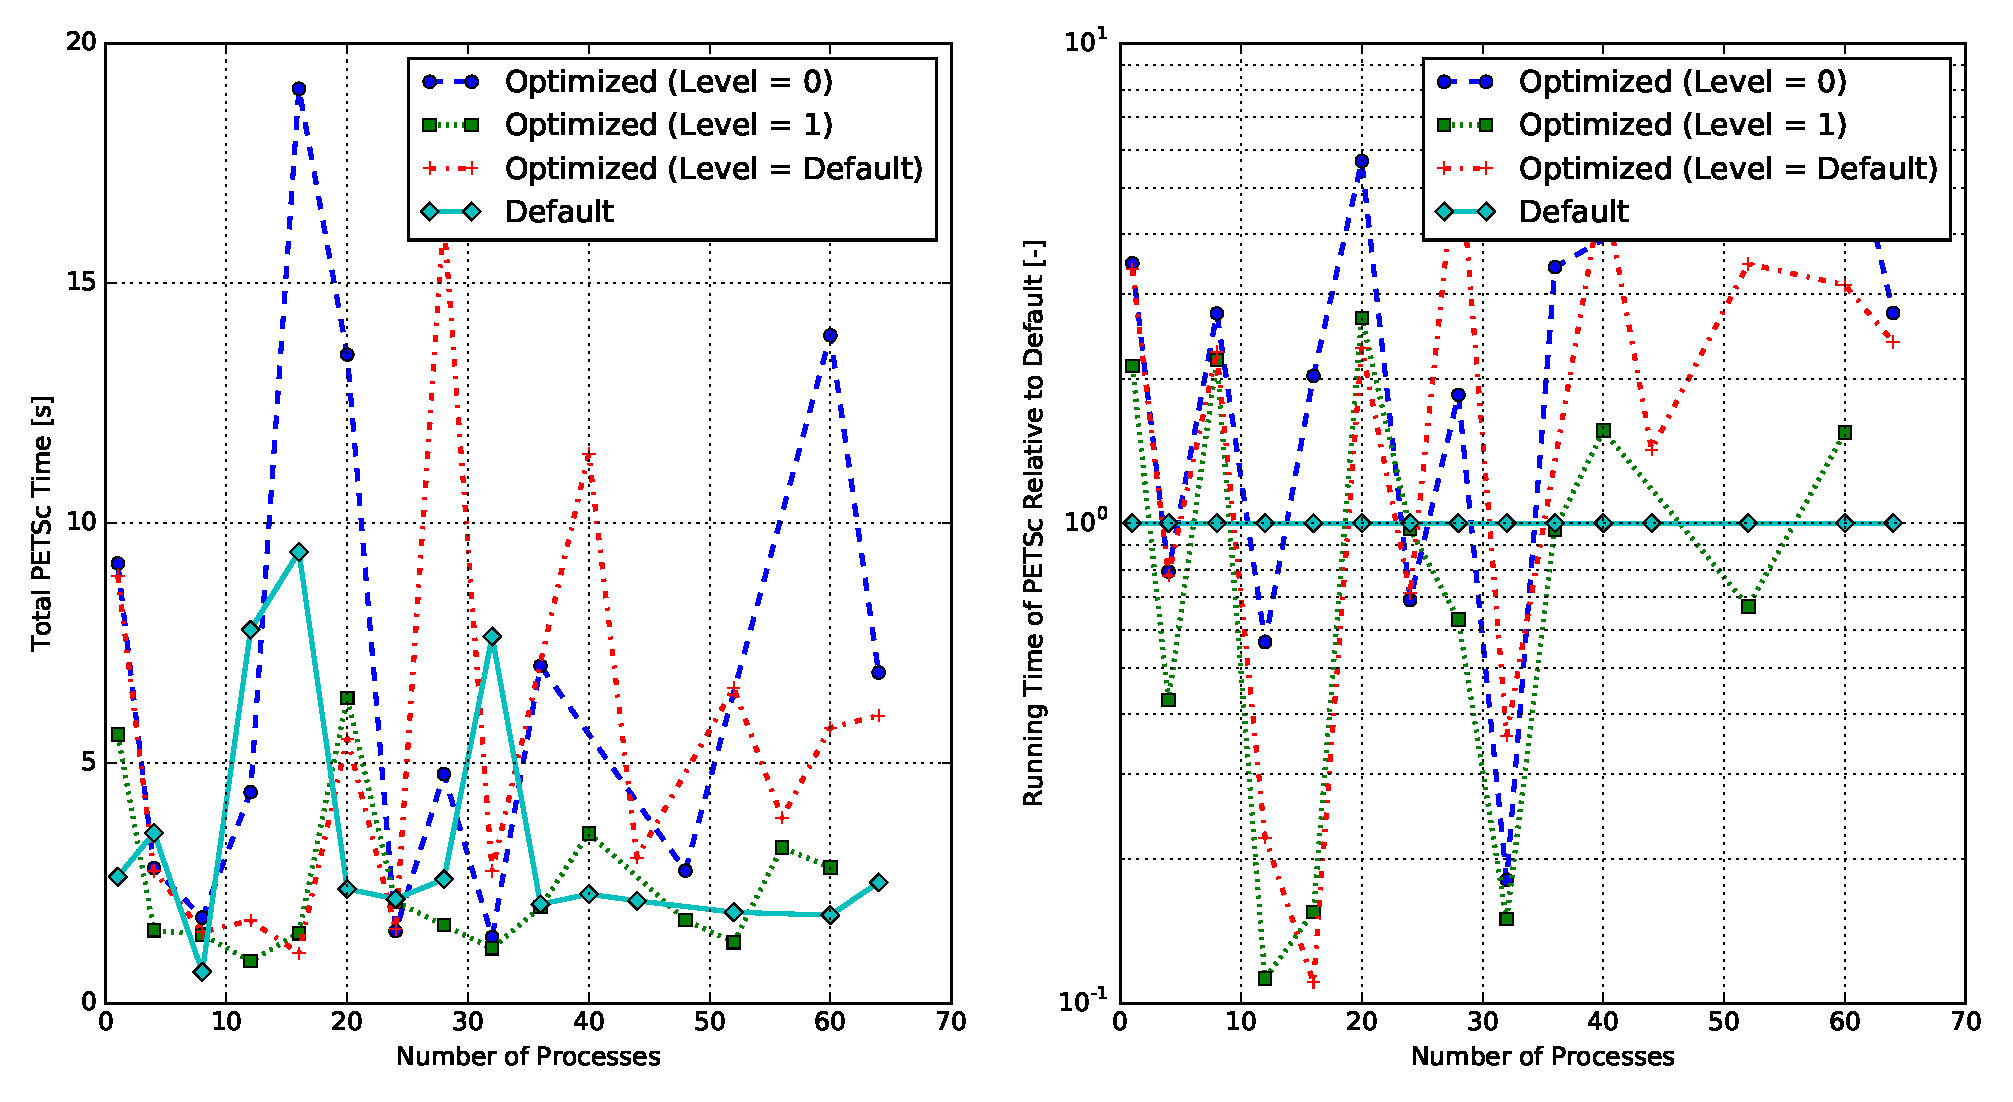
\includegraphics[width=\textwidth]{FIGURES/petsc-optimization/256x64-laminar.eps}
  \caption{Scaling test for the laminar case on a $256 \times 64$ grid}
  \label{fig:petsc-opt-scaling-laminar-256}
\end{figure}

\begin{figure}[h]
  \centering
  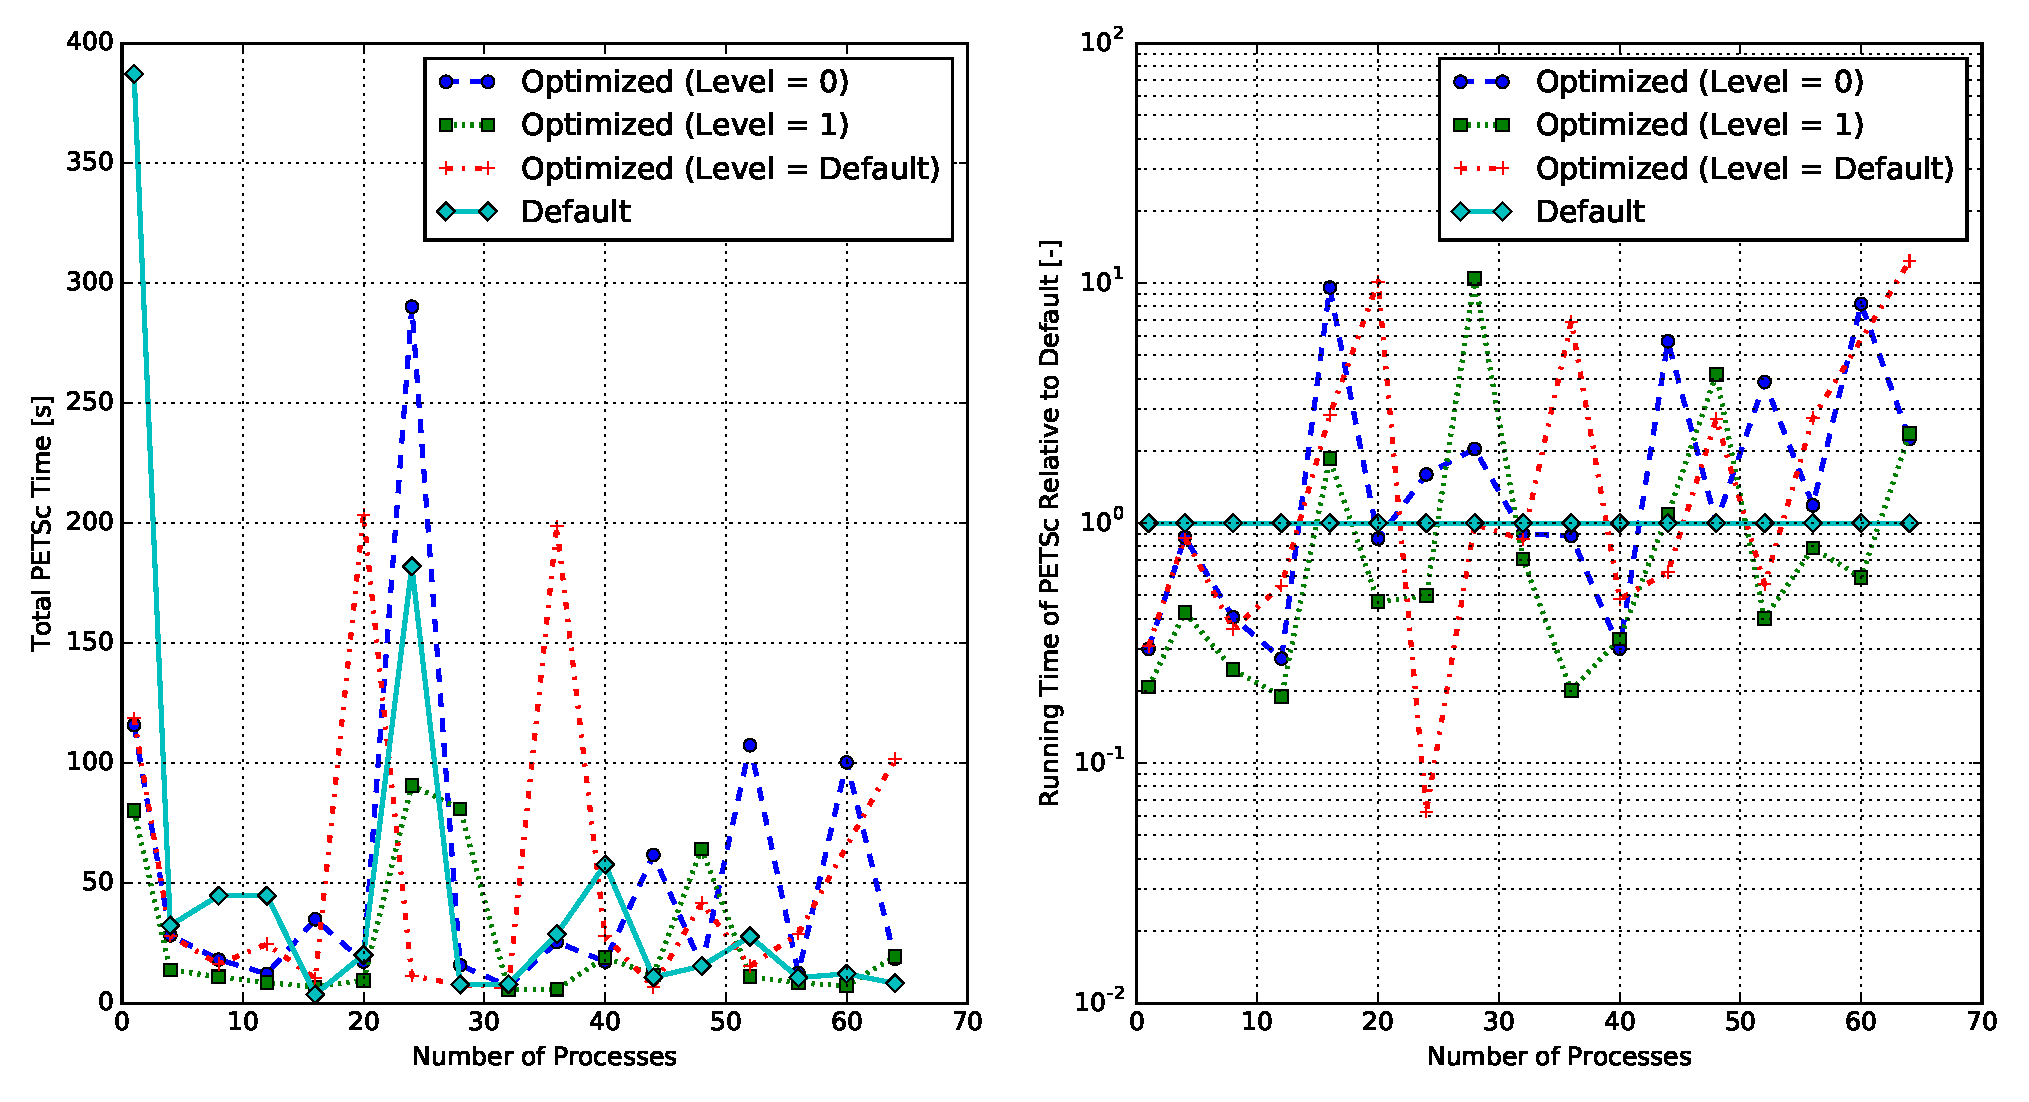
\includegraphics[width=\textwidth]{FIGURES/petsc-optimization/512x128-laminar.eps}
  \caption{Scaling test for the laminar case on a $512 \times 128$ grid}
  \label{fig:petsc-opt-scaling-laminar-512}
\end{figure}

\begin{figure}[h]
  \centering
  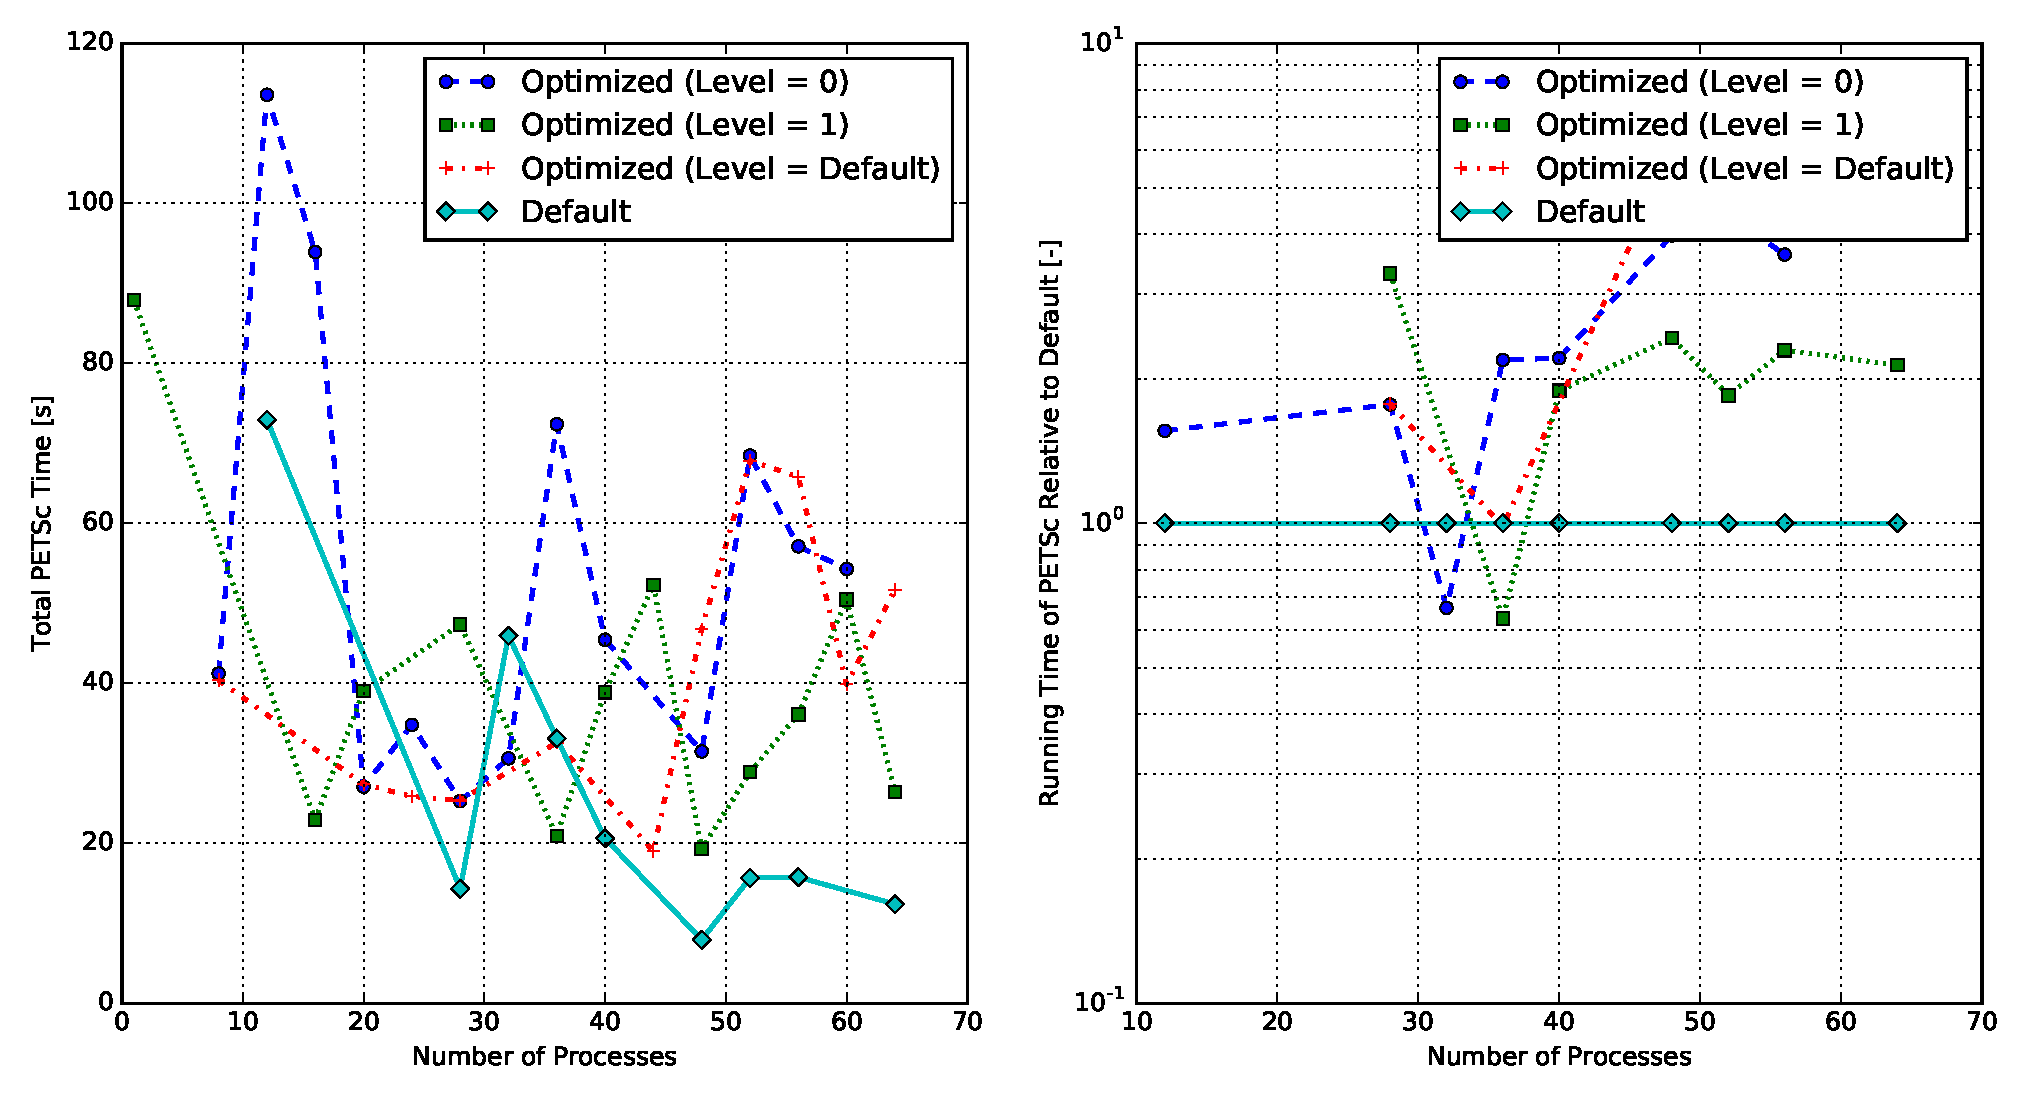
\includegraphics[width=\textwidth]{FIGURES/petsc-optimization/256x64-algebraic.eps}
  \caption{Scaling test for the algebraic case on a $256 \times 64$ grid}
  \label{fig:petsc-opt-scaling-algebraic-256}
\end{figure}

\begin{figure}[h]
  \centering
  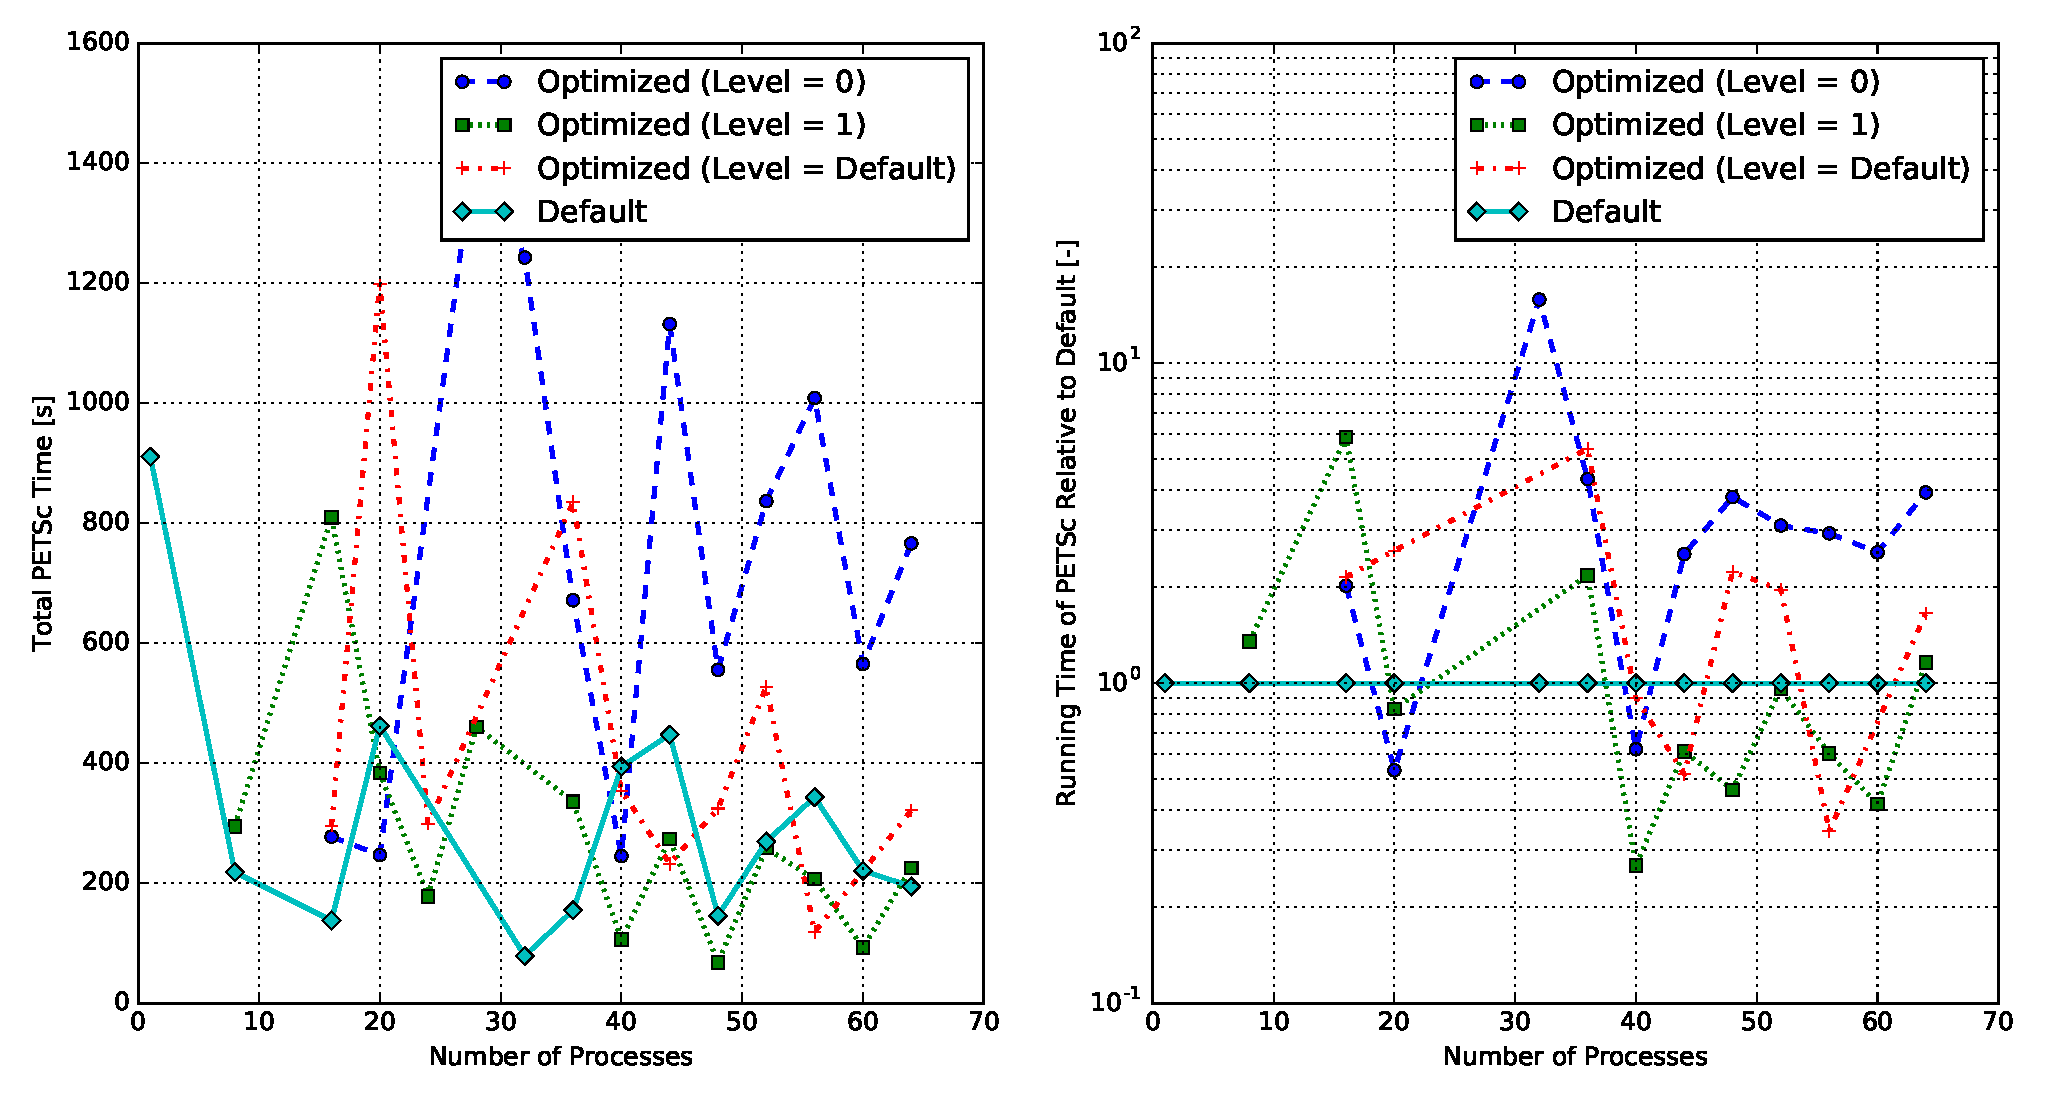
\includegraphics[width=\textwidth]{FIGURES/petsc-optimization/512x128-algebraic.eps}
  \caption{Scaling test for the algebraic case on a $512 \times 128$ grid}
  \label{fig:petsc-opt-scaling-algebraic-512}
\end{figure}

% chapter performance_tests (end)

\chapter{Binary Data Output with HDF5 and MPI-IO}
\label{cha:hdf5}

The original VTK output implemented within the scope of worksheet 1 is easy to
implement and debug because it allows for inspection of the data with any text
editing program. But at the same time it treats time and space wastefully by
requiring a conversion to ASCII and using separator characters instead of a
fixed-width format. Storing a double precision floating point value in a VTK
file requires a conversion from binary data to ASCII string which takes time
while also reducing the precision. Our current VTK writer generates ASCII
representations of 8 characters length, which gives you a best case precision of
7 digits for numbers like $1.234567$ because you have to subtract one byte for
the dot and can only keep 6 decimal places. A number like $2.33 \cdot 10^{-5}$
is truncated to $0.000002$ leaving only a single digit intact.

A binary, fixed width format does away with these disadvantages at the cost of
inspectability. Data can be written directly from memory without requiring a
relatively costly transformation and you keep all the benefits of IEEE floating
point numbers. So you can fit a precision 16 decimal places into the same 8
bytes that gave you only 6 decimal places with VTK.

First we looked into the library version of VTK that implements a new version 2
of the VTK format with several interesting features, for example support for
binary output but also built-in support for multiple writers. Sadly this
foundered on that fact that documentation for this library is very sparse
without a commercial subscription with KitWare. Additionally their plan for
parallelism consists of every process writing its own file and linking them
together with an index file and we were also looking for a way to have everyone
write into the same file.

This led us to HDF5 \footnote{https://www.hdfgroup.org/HDF5/}, the Hierarchical
Data Format. This format has basically all the features we wished for.

\begin{itemize}
\item HDF5 is a binary format
\item It has support for MPI built-in
\item Everyone writes into the same file
\item It is very well documented
\end{itemize}

There is unfortunately a unavoidable drawback in that this
format alone is not directly understandable by visualizers like ParaView because
HDF5 files are more or less file systems of arbitrary structure in a file. Thus,
another program cannot make sense of the data without some kind of description
of the structure. The solution to this problem is called XDMF, Extensible Data
Model and Format \footnote{http://xdmf.org/index.php/Main\_Page}, which
describes the structure of HDF5 files and lets you communicate facts like
``/Data/Timestep-1/Pressure'' is the pressure data at timestep 1 to ParaView.

Nonetheless this enabled us to implement a binary data output where all
processes write into the same file using MPI-IO under the hood.

\infobox{nseof::hdf5::HDF5, nseof::hdf5::XDMF, nseof::hdf5::HDF5Plotter}

In beginning all processes collectively create an output file and then write
there local flow field geometry into it. Then every $n$ timesteps all processes
write all their plotting data into the binary file, e.g. the current pressure or
dissipation rate. This requires some synchronization overhead to ensure that all
data is actually written. In practice this means that all processes need to
write their data collectively, i.e. process 1 needs to know where process 3 is
writing its data. It does not have to wait for it (i.e. non-blocking), but has to
know about it. If you try to drop this mapping, you will find that parts
of the HDF5 output are missing. Finally all processes close the HDF5 file and
the root process generates an XDMF description for ParaView.

This improvement reduced the output file size by about 35\%. This is about what
you would expect. When you read back to the first paragraph, you see that all
the double values are still taking 8 bytes of storage space, the same as
before. So effectively we only save the field separators and the local field
geometries that are repeated in every VTK file. You also have to take into
account the double values that we save now have more than double the amount of
precision. In the end this means that while we only saved approximately 35\% of
space, we increased the information density of our output by a factor of
$\frac{1}{65\%} \cdot \frac{16}{7} \approx 3.5$ where $\frac{1}{65\%}$ is the
information density of the binary output and $\frac{16}{7}$ is the increase of
information by increasing the precision from $7$ to $16$ decimal places.

\section{Limitations}

Unfortunately there are two limitations that could not be resolved.

\begin{itemize}
\item There is no currently no combination of modules on the MAC-cluster that
  allows the successful compilation with HDF5 enabled
\item ParaView is not able to read/understand vector data
\end{itemize}

Our analysis of the first issue revealed that there the HDF5 module is compiled
with multi-threading enabled while the MPI module version that we have to use
because of other inter-module dependencies is compiled without multi-threading
support (or the other way around). This leads to unresolvable inconsistencies
during the linking process.

Regarding the second issue it is not clear who the offender is. Are we writing
invalid XDMF files or is there a bug in ParaView respectively libxdmf? That is
not easy to answer because in contrast to HDF5 XDMF is maintained and developed
by KitWare which means that, like VTK, useful documentation or even working
examples of XDMF are few and far between. We were simply unable to find even one
working example how to correctly describe vector data.

\chapter{Numerical results of DNS Simulations} % (fold)
\label{cha:numerical_results}

\section{Backward facing step} % (fold)
\label{sec:backward_facing_step}

Josef

% subsection backward_facing_step (end)

\section{Karman vortex street - flow around a cylinder in a channel} % (fold)
\label{sec:karman_vortex_street_flow_around_a_cylinder_in_a_channel}

Peter

% subsection karman_vortex_street_flow_around_a_cylinder_in_a_channel (end)

% chapter numerical_results (end)
\chapter{Instrumentation with ScoreP}
\label{cha:scorep}

\section{Introduction}

Parallel computing can be complex when working with large programs. In order to
get a better overview of a programs behavior and possible inefficiencies, many
instrumentation packages have been produced to aid developers in finding
bottlenecks in their code. Instrumentation refers the insertion of pragmas into
an existing code the monitor the codes behavior at runtime and saves a record
for latter review. Although instrumentation can be useful, it should be noted
that when instrumentation is inserted into code, it may cause changes in
performance. These changes can be due to changes in memory allocation due to
the instrumentation's presence and can also cause Heisenbugs, or the change in
a program's behavior when trying to observer it. The two main types of
instrumentation are profiling and tracing. Profiling describes the measurement
of the duration or frequency of function calls. This can be very useful in
gaining an overview of a programs characteristic, and discovering
computationally intensive hotspots. Profiling is fairly inexpensive and can
provide a moderate amount of performance data. What profiling does not excel in
is displaying the chronological order of events relative to one another. For
this purpose, tracing is better suited. Tracing can be used to recreate and
study dynamic program behavior after program execution has completed. Tracing
logs event information about a programs execution and communication at run
time. Events usually consist of timestamps and process ids as well as process
specific data. These event logs can be very large in size and are written to a
memory buffer during execution, and must be flushed (written to disk) when the
buffers fill. For this reason, tracing can more heavily influence the execution
of program when improperly implemented. Both tracing and profiling can be
helpful when looking to find performance bottlenecks in parallel code, and when
used together can be very powerful. One large instrumentation package developed
in Germany is ScoreP.

ScoreP is a compiler wrapper that allows developers to take advantage of
multiple instrumentation tool like Vampir, Cube, and Scalasca while using only
one compiler wrapper. By setting environment variables, the user can easily turn
functionalities on and off at runtime.

\section{Goals and Approach}

Our goals for our code analysis were to identify excessive communication,
frequent synchronization and load balancing issues. To analyzing our code, we
first profiled the code and analyzed the results in Cube. This allowed us to get
an overview of the computationally intensive processes and assess weather or not
we would like to filter out. When not using a filter file, the flush points were
manageable for low scale simulations but became more disturbing as the
simulations became large. We then implemented a filter for the Petsc solve
directory to solve this issue.

We were then able to confidently activate tracing and run another
simulation. When viewing the trace data in figure \ref{fig:scorep-trace-data},
one can see that after MPI initialization, the computational intensity of our
simulation is relatively high. The largest load-imbalance and synchronization
issue when calling MPI allreduce, which arises on vtk write iterations.

\begin{figure}[h]
  \centering
  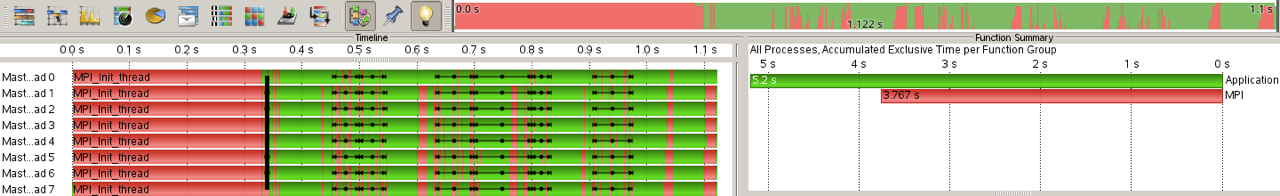
\includegraphics[width=\textwidth]{FIGURES/scorep/trace-data}
  \caption{Nodes waiting for one another during VTK output}
  \label{fig:scorep-trace-data}
\end{figure}

This can most likely be attributed to the bottleneck at the disk when outputting
the VTK files. This phenomenon was removed after the vtk output was
deactivated. With the VTK output turned off, the computational intensity was
consistently high.

\begin{figure}[h]
  \centering
  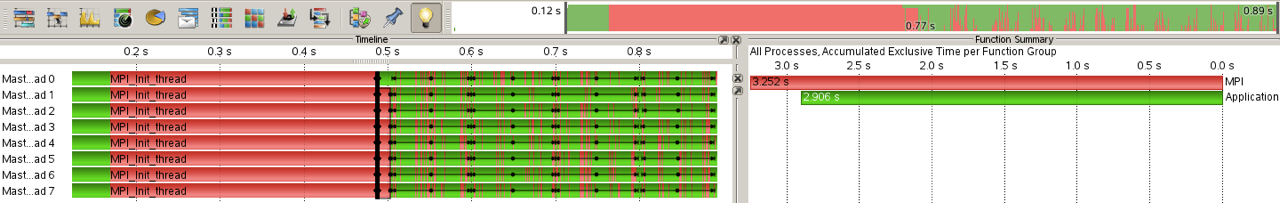
\includegraphics[width=\textwidth]{FIGURES/scorep/reference}
  \caption{Trace showing high computational intensity}
  \label{fig:scorep-reference}
\end{figure}

This could be supplemented with a parallel file access system which was not
present during this simulation. With figure \ref{fig:scorep-reference} the rest
of the computation has a considerably high computational intensity, that we are
very pleased with.

\chapter{Tooling \& utilities}
\label{cha:tooling}

Over the course of this semester we adopted several tools, restructured the code
quite a bit and programmed several utilities to keep the software organized and
automize recurring tasks.

\section{Code quality}

\subsection{Namespaces}

After the second worksheet there were slightly different versions of several
classes right next to each other and it became hard to keep track of what
belonged together. To better emphasize, which classes are coupled closely
together, we grouped them classes into namespaces. First and foremost all code
now lives under the \texttt{nseof} namespace. Inside of this we divided the code
into

\begin{itemize}
\item \texttt{flowmodels} to group all classes related to flow modelling with
  subnamespaces \texttt{laminar} for the base case, \texttt{turbulent} with
  parent classes for all turbulence models, \texttt{algebraic} for the algebraic
  model from the second worksheet and \texttt{ke} for the $k$-$\epsilon$
  turbulence model
\item \texttt{hdf5} for HDF5 data output
\item \texttt{walldistance} for computing the wall distance of a cell with ANN
\item several more
\end{itemize}

\subsection{Coding Style \& formatters}

Keeping a consistent coding and formatting style throughout a codebase helps
keeping the code readable and even find bugs. Therefore we first agreed on a
well-defined coding style to adhere to, in our case the one maintained by Google
\footnote{http://google.github.io/styleguide/cppguide.html} because it had the
most familiarity to how you program in Java.

Secondly we configured the C++ code formatter clang-format to adhere to this
style, so that we could automatically reformat the existing codebase and also
check the style of newly written code before committing it into our repository.

\section{Tools}

Most importantly we replaced the original Makefile with CMake
\footnote{https://cmake.org/}. CMake lets you easily script different aspects of
your build. For example we implemented an option to use the special MPI compiler
on the MAC cluster, another one to enable profiling with gprof and a another one
to enable instrumentation with scorep, so that you can configure all those
things command line switches instead of having to edit the Makefile. However the
most important feature for us was that CMake has working dependency checking so
that you can always just make and CMake will figure out, exactly which files
need to be recompiled. This presents a remarkable saving of time compared to the
original Makefile, where this was not guaranteed to work.

Secondly we integrated Google's GTest
\footnote{https://github.com/google/googletest} into our CMake configuration and
created several tests to check the correctness of several of the derivative
functions.

\section{Utilities}

We developed a few utilities to simplify tasks and shrink multi step processes
into a single command.

\subsection{Connecting to the cluster}

Whenever you want to run a simulation with a lot of cores you need to log on to
the MAC cluster. But this is not so straight forward since the MAC cluster is
only available inside the TUM network. This means you have to tunnel into
university network and then connect throught that. All these things are managed
by the following script, so that you do not have to care.

\bashh{FIGURES/tooling/connect}{1}

Additionally it can also mount your home and scratch directory.

\subsection{Running jobs}

There is a \texttt{run} script that configures batch jobs and queues them. It is
fully controlled by command line arguments so that you never have to edit
files. The following call runs the scenario \texttt{scenario.xml} with
$8 \times 2$ processes on intel nodes with a maximum run time of 30 minutes,
puts the results into \texttt{./results} and sends you an email, when it is
done.

\bashh{FIGURES/tooling/run}{1}

If you pass \texttt{-l} or \texttt{--local}, you can also use it on your own computer.

\subsection{Performing scaling tests}

The \texttt{scale} script performs a weak or strong scaling experiment for
you. For example the following command would test strong scaling with the
scenario \texttt{scenario.xml} on intel nodes with a grid size of
$512 \times 64$ with $1, 4, 8, \dots, 64$ processes and put all results into
\texttt{./results} for later analysis with one of the analysis and plotting
scripts.

\bashh{FIGURES/tooling/scale}{1}

An interesting feature of this script is that it computes the optimal domain
decomposition automatically for all numbers of processes that should be
tested. In the lecture we established that an optimal decomposition consists of
rectangles with a minimal ratio of surface area to volume because that is
actually the same as the ratio of communication to computation.

Say you want to run a $k$-dimensional simulation with $n$ cores on a domain with
$s_{1} \cdot s_{2} \cdots s_{k}$ cells. Then we have to decompose $n$ into
$n_{1}, \dots, n_{k}$ such that $\prod_{i = 1}^{k} n_{k} = n$. This means that
all the $n_{i}$ have to be divisors of $n$ or more specifically all $n_{i}$ have
to be either $1$ or a product of the prime divisors of $n$. Let
$\mathcal{P}_{n}$ be the set of all prime divisors of $n$ with correct
multiplicity. Furthermore let $\mathcal{C}_{n}$ be the set of all ordered
products of $k$-partitions of $\mathcal{P}_{n}$. For example for $k = 3$ we have
$\mathcal{P}_{12} = \{ 2, 2, 3 \}$ and
\begin{equation*}
  \mathcal{C}_{12} = \{ (12, 1, 1), (1, 12, 1), (1, 1, 12), (4, 3, 1), (4, 1, 3), (3, 4, 1), \dots \}
\end{equation*}
Let $(n_{1}, \dots, n_{k}) \in \mathcal{C}_{n}$ be a decomposition. This
decomposition divides the domain into parts of surface area $A$ and volume $V$
where
\begin{equation*}
  A = 2 \cdot \sum_{i = 1}^{k} \prod_{j = 1, j \ne i}^{k} \frac{s_{j}}{n_{j}} \qquad \textit{and} \qquad V = \frac{1}{n} \prod_{i = 1}^{k} s_{i}
\end{equation*}
Now remember that we are trying to minize the ratio of surface area to volume,
i.e.
\begin{align*}
  \frac{A}{V} & = \frac{n}{\prod_{i = 1}^{k} s_{i}} \cdot 2 \cdot \sum_{i = 1}^{k} \prod_{j = 1, j \ne i}^{k} \frac{s_{j}}{n_{j}} = \frac{n}{\prod_{i = 1}^{k} s_{i}} \cdot 2 \cdot \sum_{i = 1}^{k} \frac{\prod_{j = 1, j \ne i}^{k} s_{j}}{\prod_{j = 1, j \ne i}^{k} n_{j}}\\
  & = 2 \cdot \sum_{i = 1}^{k} \frac{\prod_{j = 1, j \ne i}^{k} s_{j}}{\prod_{i = 1}^{k} s_{i}} \cdot \frac{n}{\prod_{j = 1, j \ne i}^{k} n_{j}} = 2 \cdot \sum_{i = 1}^{k} \frac{1}{s_{i}} \cdot n_{i} = 2 \cdot \sum_{i = 1}^{k} \frac{n_{i}}{s_{i}}
\end{align*}
Minimizing this analytically is not trivial since we have to find solutions on a
$k - 1$-dimensional submanifold that is described by a non-linear equation
($\prod_{i = 1}^{k} n_{i} = n$). You can however work out special cases
directly. Let for example be $k = 2$.
\begin{equation*}
  \frac{A}{V} = 2 \cdot \left( \frac{n_{1}}{s_{1}} + \frac{n_{2}}{s_{2}} \right) = 2 \cdot \left( \frac{n_{1}}{s_{1}} + \frac{n}{n_{1}s_{2}} \right) \qquad \left( \frac{A}{V} \right)' = 2 \cdot \left( \frac{1}{s_{1}} - \frac{n}{s_{2} n_{1}^{2}} \right)
\end{equation*}
where the derivative with respect to $n_{1}$ has a root at
$n_{1} = \sqrt{\frac{ns_{1}}{s_{2}}}$. Though you are still not done, because
you have to find the closest integer approximation to
$\left( n_{1}, \frac{n}{n_{1}} \right)$.

That is why the script uses a different algorithm to construct the same integer
solutions directly. It is based on the observation that the subdomains will be
squares when it holds for all $i, j$ that
$\frac{s_{i}}{s_{j}} = \frac{n_{i}}{n_{j}}$, i.e. the number of cores along some
dimensions have the same ration as the number of cells along these dimensions,
because then the subdomains will be $k$-dimensional squares. The integer
solution is constructed iteratively by starting with a decomposition of
$(n_{1}, \dots, n_{k}) = (1, \dots, 1)$ and then multiplying the prime factors
in descending order onto the $n_{i}$ whose ratio of $\frac{n_{i}}{s_{i}}$ is
minimal because that is the one that is the furthest away from its optimal
value, i.e. having the same ratio as all other $n_{i}$. Table
\ref{fig:tooling-decompositions} shows a few example decompositions obtained in
this manner.

\begin{table}[h]
  \centering
  \begin{tabular}{c|cc}
    \hline
    $n$ & $n_{1}$ & $n_{2}$\\
    \hline
    1 & 1 & 1\\
    4 & 4 & 1\\
    8 & 8 & 1\\
    12 & 6 & 2\\
    16 & 8 & 2\\
    20 & 10 & 2\\
    24 & 12 & 2\\
    28 & 14 & 2\\
    32 & 16 & 2\\
    36 & 9 & 4\\
    \hline
  \end{tabular}
  \caption{2-dimensional decompositions of a domain with $512 \times 128$ cells for $n$ processes}
  \label{fig:tooling-decompositions}
\end{table}

Finally the script mangles the cell counts $s_{1}, \dots, s_{k}$ just a little
by rounding up or down to the next multiple of $n_{k}$ so that $n_{k}$ divides
$s_{k}$ because the simulation only accepts decompositions that divide the
domain into parts of exactly equal size.

%!TEX root = ./../projectReport.tex

\chapter{Usability} % (fold)
\label{cha:usability}
To perform the commands shown in this chapter, please navigate to the C++-project folder ('turbulence').


\section{Project folder} % (fold)
\label{sec:project_folder}

NS-EOF can still be run by writing into the shell the following command:

\bashh{SCENARIOS/run.txt}{1}

\noii However, we advice to run the Python-script 'run' both on the cluster and locally to start the simulation\footnote{For more information on the options, we refer to the help:
\bashh{SCENARIOS/runh.txt}{1}
}:

\bashh{SCENARIOS/runl.txt}{1}

\noii By doing so, the simulation is started, but also a new folder is created containing all relevant files of the simulation. This folder is referenced in the following as project folder.

\noii By copying and placing all the input files (configuration file, backup file for initialisation, geometry file) and all the result files (output, VTK files, backup file, timing results) into one folder, the user is enabled to completely understand the simulation at a later time.

\noii The following tree shows the structure of the project folder:
\dirtree{%
.1 project.
.2 job.cmd.
.2 log.
.2 out.
.2 petsc\_commandline\_arg.
.2 scenario.xml.
.2 timing/.
.3 ....
.2 vtks/.
.3 ....
}

\noii The next sections describe two input files (the configuration and the geometry files) in more detail.

\clearpage

\section{Configuration file} % (fold)
\label{sec:configuration_file}

For the sake of completeness, a configuration file is shown in its original appearance as provided at the beginning of the lab course. 

\noii It contains the setup for a DNS simulation of a backward facing step scenario with a streched mesh.

\xmll{SCENARIOS/conf-reference.xml}{2}

\noii All additional new options are shown in the following sections in reference to this file.

\noii \textbf{Tested configuration files} can be found in the 'scenarios'-folder.

\newpage
\subsubsection*{Algebraic turbulence model}

For the second worksheet, the group implemented an algebraic turbulence model with different methods to limit the mixing length and thus the eddy viscosity (nulimiter=1: no limitation; =3 limitation with the help of a laminar flat plate Blasius boundary layer; =4 limitation with the help of a turbulent flat boundary layer). 

\xmll{SCENARIOS/type-aturb.xml}{2}

\noii A laminar simulation with this implementation can be performed by setting $\nu_t$ to zero (type='laminar'). The results should be comparable with the DNS-simulation (\citep{lienen2015} p.~14).  

\subsubsection*{\ke\,turbulence model}

The user can use alternatively to the algebraic turbulence model the k-$\varepsilon$ model to calculate the eddy viscosity. Following optional parameters can be set:
\begin{itemize}
\item model constants $C_{\varepsilon 1}$, $C_{\varepsilon 2}$, $\sigma_k$, $\sigma_\varepsilon$ and $C_{\mu}$ (see equation~\ref{equ:constants})
\item wall near treatment (model=0: no wall modifications, =1: Lam and Bremhorst, =2: Chien, =3: Jones and Launder, =4 Fan and Lakshminarayana)
\item adaptive time stepping (number of refinements and permitted errors)
\item solving quasi laminarly for the first 'start' seconds (not solving the transport equations for $k$ and $\varepsilon$ and setting $\nu_T=0$)
\end{itemize}

\xmll{SCENARIOS/type-ke.xml}{2}

\noii A laminar simulation with this implementation can be performed by setting $\nu_t$ to zero (type='laminar').

\subsubsection*{Scenarios}

As described in section~\ref{sec:new_scenarios}, following scenarios were added:

\begin{itemize}
\item symmetrical channel
\xmll{SCENARIOS/scenario-channel-symm.xml}{1}
\item boundary layer over a flat plate
\xmll{SCENARIOS/scenario-boundary.xml}{1}
\item free shear flow (without any side walls)
\xmll{SCENARIOS/scenario-free.xml}{1}
\end{itemize}

\subsubsection*{Inlet}

For every scenario except for 'cavity', the velocity inlet profile in x-direction can be prescribed as either uniform (true) or parabolic (false).

\xmll{SCENARIOS/scenario-uniform.xml}{1}

\subsubsection*{Flow around arbitrary geometry}

The user can specify a reference to a geometry file (see: \ref{sec:geometry_file}) to be used to set up an obstacle in any scenario.

\xmll{SCENARIOS/ageom.xml}{2}



\subsubsection*{Backup files}

The user can specify the backup (.bak) files to be used for initialisation and for saving the results of the final time step. Backup files are written after every interval specified by the user and at the end of the simulation.

\xmll{SCENARIOS/restart.xml}{2}

\noii No file ending '.bak' needs to be specified in the configure file.

% subsection configuration_file (end)

\clearpage

\section{Geometry file} % (fold)
\label{sec:geometry_file}

The geometry file (.geo) contains the coordinates of all obstacle cells. Each line represents exactly one obstacle cell and has the following format (with the first number i, the second number j and the third number k):

\xmll{SCENARIOS/geo.txt}{2}

\noii The team developed two Matlab-scripts for creating files of the necessary format for 2D geometries:
\begin{itemize}
\item \underline{Scripting}:\\
The user specifies with a basic function which position is in the geometry and which is in the flow field. The Matlab-script evaluates this function for the middle point of each cell and writes the file. Elementary geometries (circle, square, plate) and geometries composed by these forms can be created:

\begin{figure}[!htb]
\centering
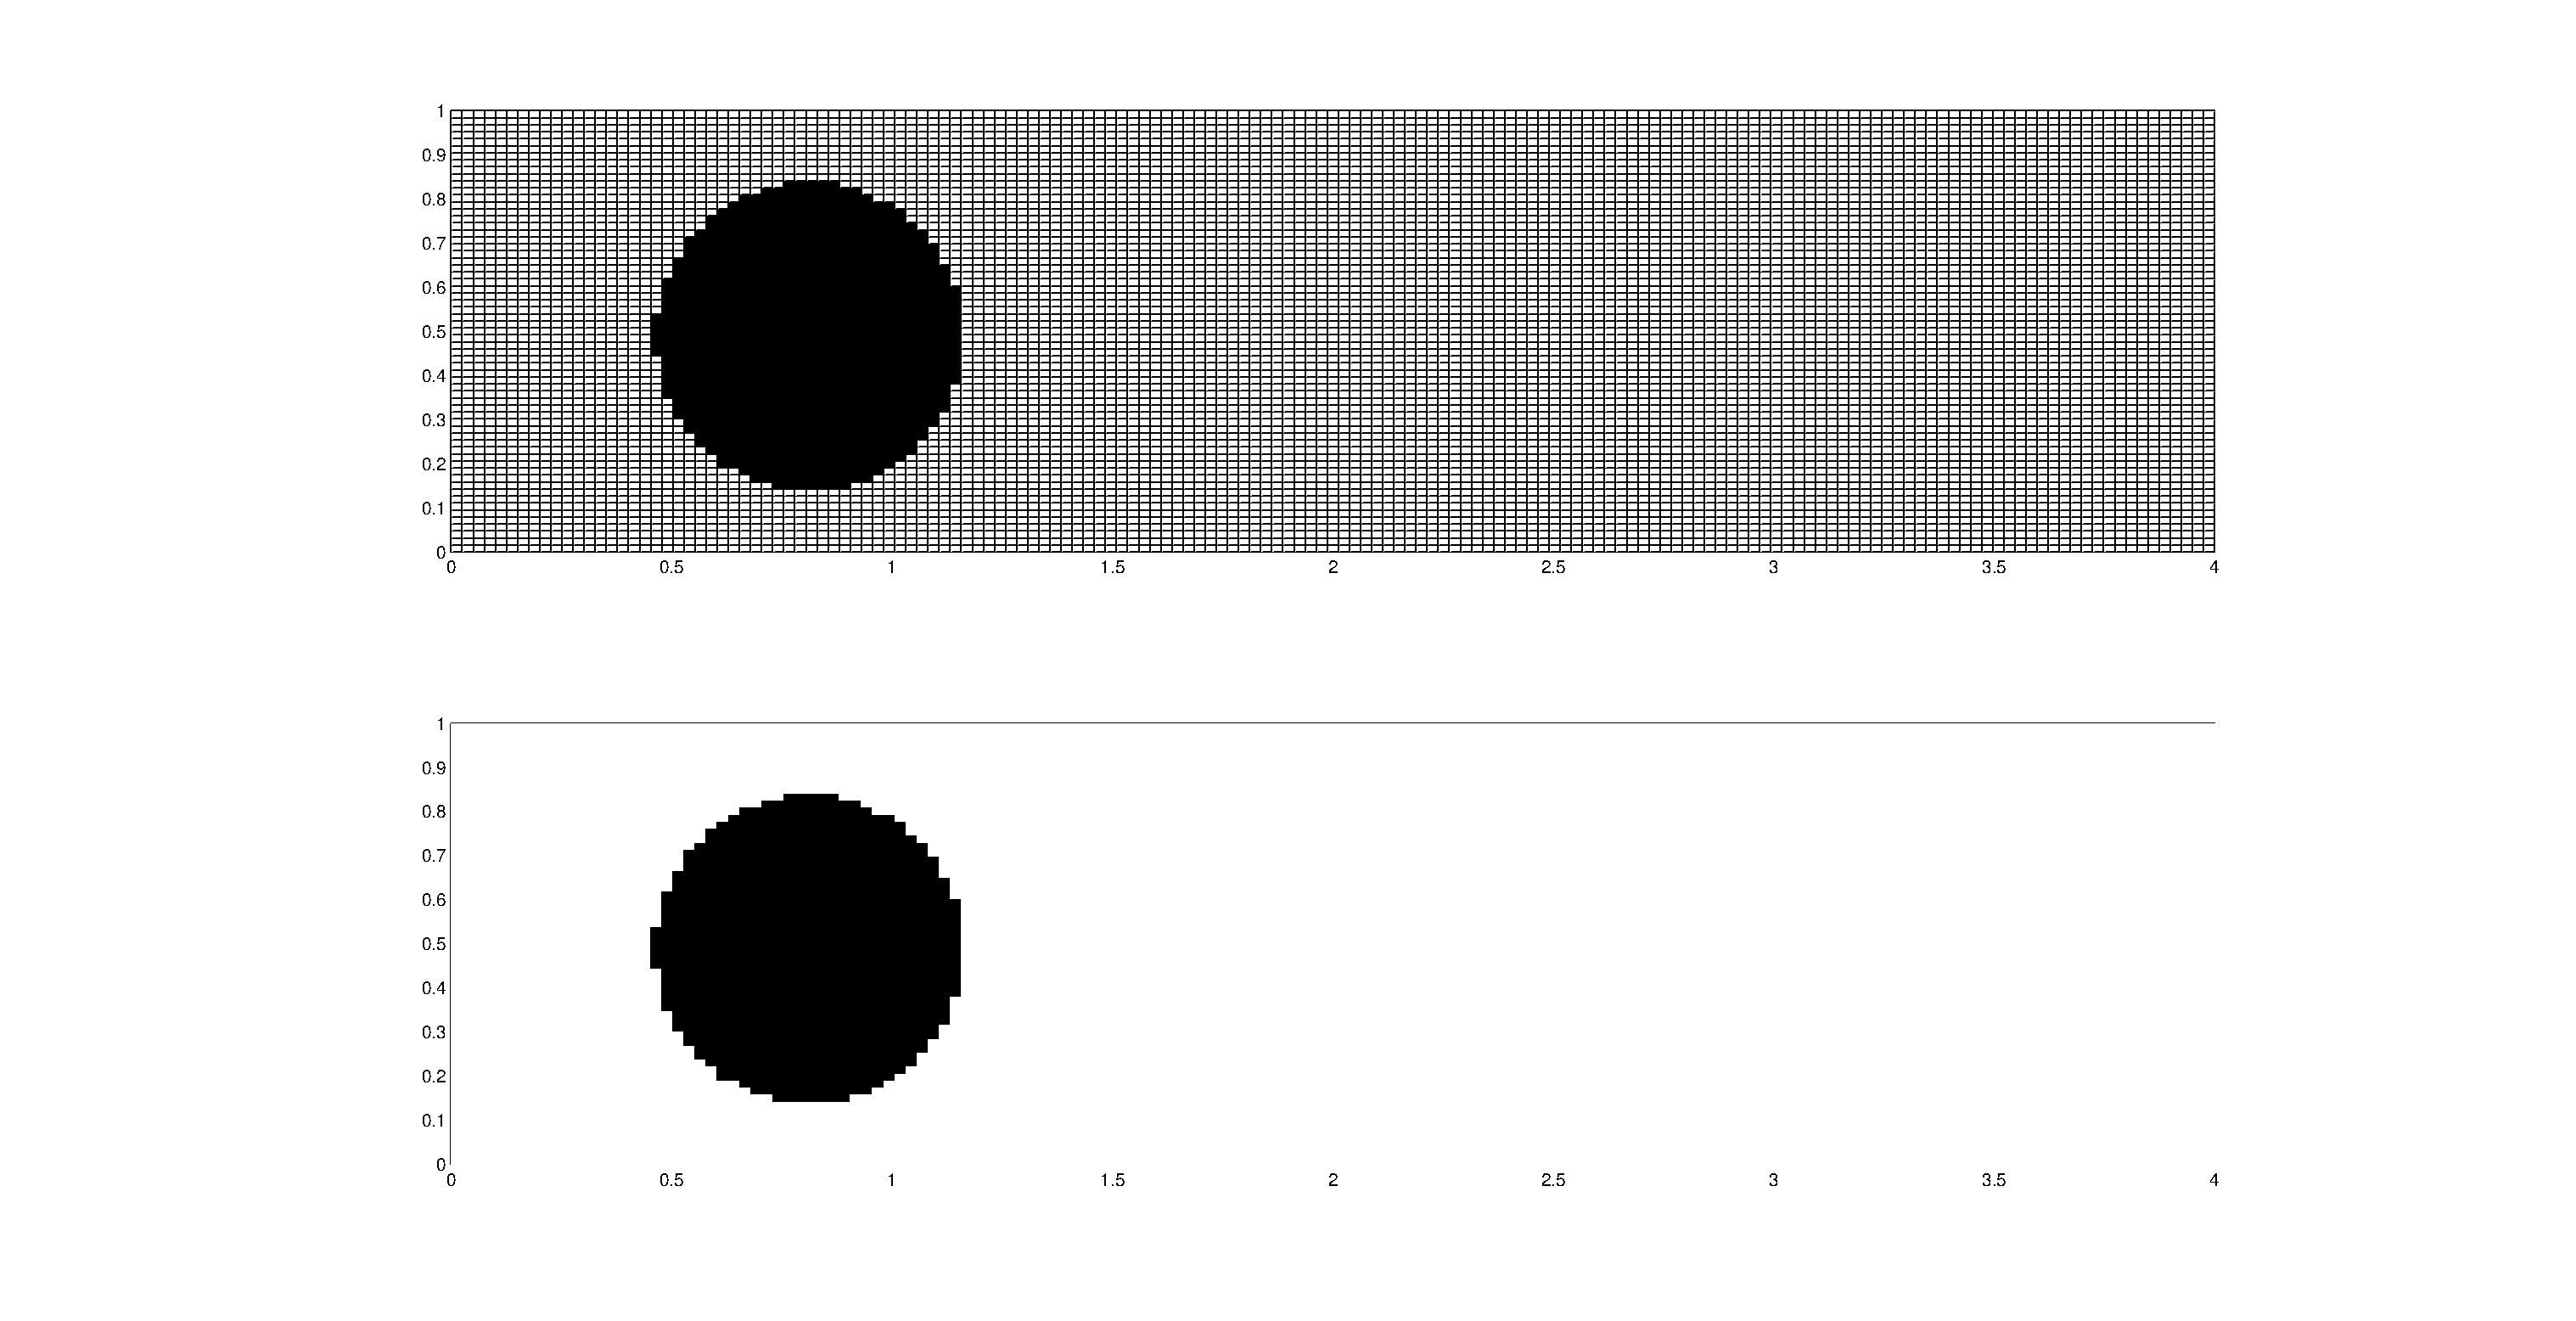
\includegraphics[scale=.3]{FIGURES/circle.eps}
\caption{Circle in a channel}
\label{fig:circle_in_channel}
\end{figure} 

\item \underline{Drag \& Drop}:\\
The second possibility to create arbitrary geometries is given by an interactive Matlab-script. The runnable script can be found in the script folder ns-eof-geogui and is called turbulence.m.
When running the script, a coordinate system with limits set according to the specified number of points in x- and y-direction shows up first. Based on this coordinate system, the surrounding line of an obstacle can be chosen.

Therefore, the starting point of the surrounding line has to be specified by a mouse click by the user\footnote{ It is recommended to keep the starting point in mind.}.
After that, the following points defining the surrounding line have to be chosen in the right consecutive order (lines between the already chosen points will show up in the coordinate frame).

To close the geometry, the point which was chosen as starting point has to be clicked again. Afterwards, the edges of the geometry can be seen in the coordinate frame.

In a next step, a point somewhere in the middle of the specified obstacle has to be clicked on. It will be used as starting point for a recursive algorithm to detect all cells lying inside the obstacle.

After this point is selected, all necessary user inputs are given and the geometry file is written in a text file.

In the figure below, an example (the created profile of an airfoil) is shown.


\begin{figure}[!htb]
\centering
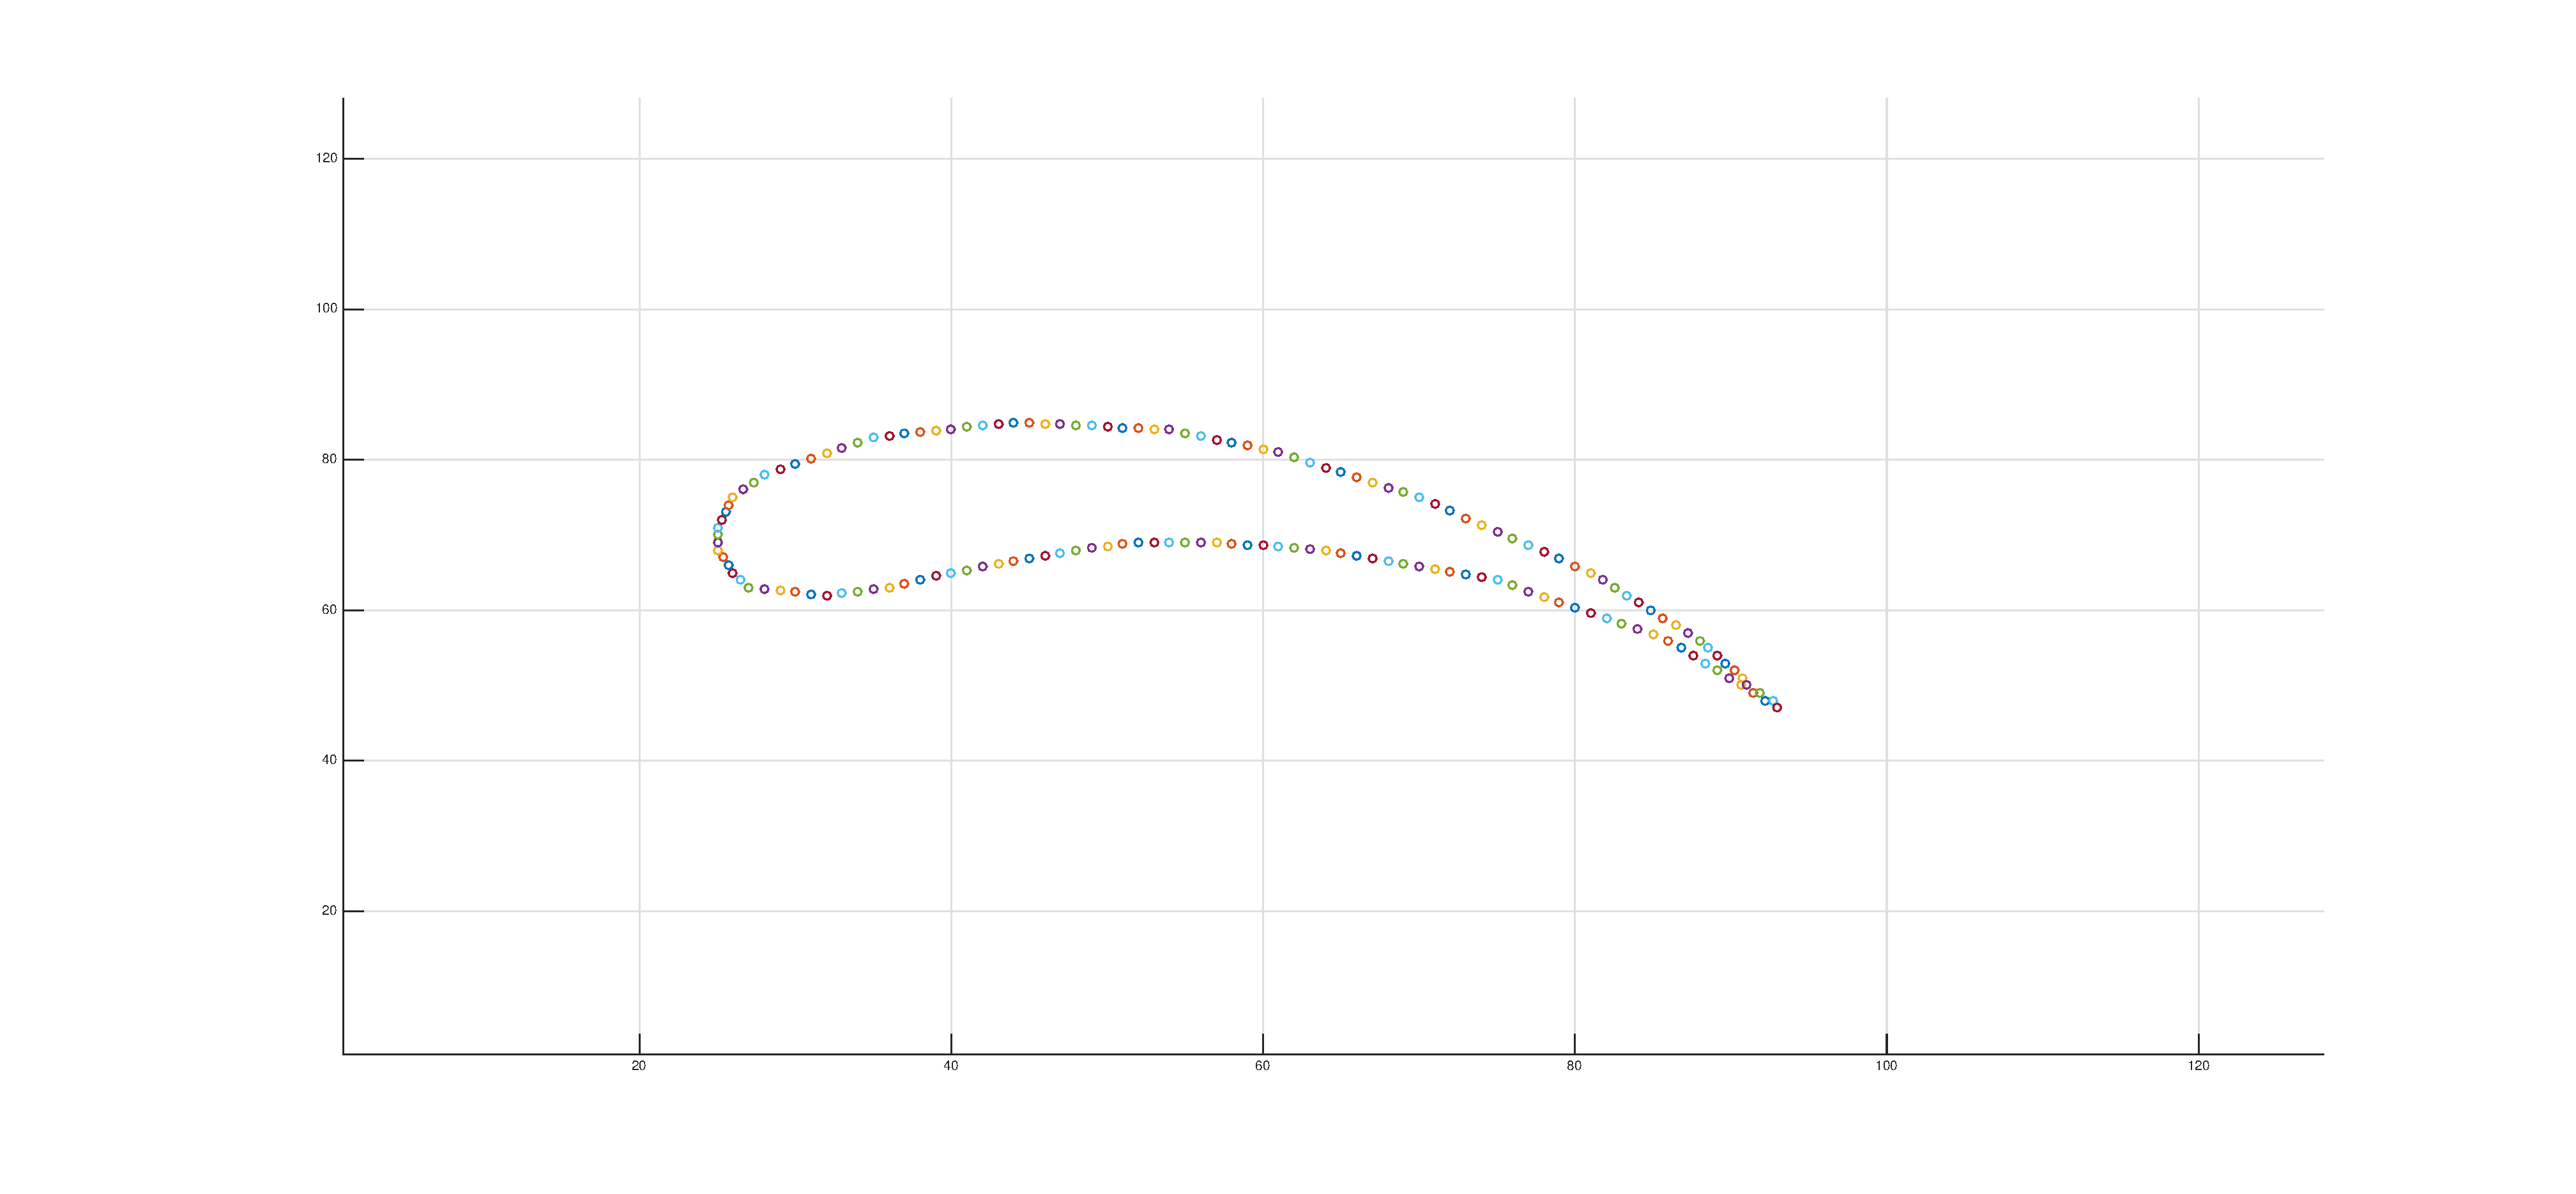
\includegraphics[scale=.23]{FIGURES/airfoil.eps}
\caption{Airfoil in a channel}
\label{fig:circle_in_channel}
\end{figure} 

\end{itemize}



% subsection geometry_file (end)

% chapter usability (end)
\chapter{Conclusion} % (fold)
\label{cha:conclusion}

% chapter conclusion (end)





\pagenumbering{roman}
\setcounter{page}{\thealteSeitenzahl}
\appendix
%\begin{appendices}

\chapter{Details Concerning Consistent Linearization of 2D Mortar Contact} % (fold)
\label{cha:details_concerning_consistent_linearization_of_2d_mortar_contact}
The computation of directional derivatives demands significant implementational effort associated with the proposed mortar finite element methods. Furthermore, they are necessary to guarantee the quadratic order of convergence of the Newton method on which the solution process is based. Due to that, details on the consistent linearizations are briefly provided in this appendix closely following \citet{popp2009}, \citet{popp2012} and \citet{farah2012}. Since this thesis restricts to the two-dimensional case, this appendix also restricts to the linearization of 2D mortar contact.

\end{appendices}

%\listoffigures
\bibliography{projectReport}{}
%\bibliography{my_bachelor_thesis}{}
\bibliographystyle{plainnat}
%\bibliography{my_bachelor_thesis}{}
%\bibliographystyle{plainnat}

\end{document}

%%%%%%%%%%%%%%%%%%%%%%%%%%%%%%%%%%%%%%%%%%%%%%%%%%%%%%%%%%%%%%%%%%%%%%%
%%%%%%%%%%%%%%%%%%%%%%%%%%%%             %%%%%%%%%%%%%%%%%%%%%%%%%%%%%%
%%%%%%%%%%%%%%%%%%%%%%%%%%%% end of file %%%%%%%%%%%%%%%%%%%%%%%%%%%%%%
%%%%%%%%%%%%%%%%%%%%%%%%%%%%             %%%%%%%%%%%%%%%%%%%%%%%%%%%%%% 
%%%%%%%%%%%%%%%%%%%%%%%%%%%%%%%%%%%%%%%%%%%%%%%%%%%%%%%%%%%%%%%%%%%%%%%